\PassOptionsToPackage{svgnames,dvipsnames}{xcolor}

\documentclass[12pt]{cmuthesis}

\usepackage[Lenny]{fncychap}
\ChNameVar{\Large}

\usepackage[%
colorlinks=true,allcolors=link_color,pageanchor=true,%
plainpages=false,pdfpagelabels,bookmarks,bookmarksnumbered,%
]{hyperref}

\usepackage[style=alphabetic,natbib=true,backend=biber,maxnames=10]{biblatex}
\bibliography{refs.bib}

\usepackage{totcount}
\newtotcounter{citenum}
\AtEveryBibitem{\stepcounter{citenum}}

\DeclareFieldFormat{citehyperref}{%
  \DeclareFieldAlias{bibhyperref}{noformat}% Avoid nested links
  \bibhyperref{#1}}

\DeclareFieldFormat{textcitehyperref}{%
  \DeclareFieldAlias{bibhyperref}{noformat}% Avoid nested links
  \bibhyperref{%
    #1%
    \ifbool{cbx:parens}
      {\bibcloseparen\global\boolfalse{cbx:parens}}
      {}}}

\savebibmacro{cite}
\savebibmacro{textcite}

\renewbibmacro*{cite}{%
  \printtext[citehyperref]{%
    \restorebibmacro{cite}%
    \usebibmacro{cite}}}

\renewbibmacro*{textcite}{%
  \ifboolexpr{
    ( not test {\iffieldundef{prenote}} and
      test {\ifnumequal{\value{citecount}}{1}} )
    or
    ( not test {\iffieldundef{postnote}} and
      test {\ifnumequal{\value{citecount}}{\value{citetotal}}} )
  }
    {\DeclareFieldAlias{textcitehyperref}{noformat}}
    {}%
  \printtext[textcitehyperref]{%
    \restorebibmacro{textcite}%
    \usebibmacro{textcite}}}


\usepackage{fullpage}
\usepackage{graphicx}
\usepackage{amsmath}
\definecolor{link_color}{RGB}{0,128,255}

\usepackage[%
letterpaper,twoside,vscale=.8,hscale=.75,nomarginpar,hmarginratio=1:1
]{geometry}

\usepackage{graphicx} % more modern
\usepackage{subfigure}

\usepackage{todonotes}
\newcommand{\todon}[1]{\todo[color=red!40,inline,size=\small]{TODO: #1}}
\newcommand{\todoc}{\todo[color=red!40,inline,size=\small]{TODO: Complete}}

\usepackage{amsmath}
\usepackage{amssymb}
\usepackage{amsthm}
\usepackage{arydshln}


\usepackage{accents}
\newcommand{\ubar}[1]{\underaccent{\bar}{#1}}

\usepackage{stackengine}

\usepackage{wrapfig}

\newtheorem{proposition}{Proposition}
\newtheorem{assumption}{Assumption}
\newtheorem{theorem}{Theorem}
\newtheorem{corollary}{Corollary}
\newtheorem{lemma}[theorem]{Lemma}

% \MakeRobust{\Call}
\newcommand*\Let[2]{\State #1 $\gets$ #2}

\definecolor{lightgray}{gray}{0.95} % 10%

\usepackage{hyperref}
\newcommand{\theHalgorithm}{\arabic{algorithm}}


\usepackage{easytable}

\usepackage[capitalise,nameinlink,noabbrev]{cleveref}

\usepackage{stmaryrd}

\usepackage{algorithm}
\usepackage{algorithmic}
% \usepackage{algpseudocode}
% \algnewcommand{\LeftComment}[1]{\Statex \(\triangleright\) #1}

\newcounter{module}
\makeatletter
\newenvironment{module}[1][htb]{%
  \let\c@algorithm\c@module
    \renewcommand{\ALG@name}{Module}%
   \begin{algorithm}[#1]%
  }{\end{algorithm}}
\makeatother
\crefname{module}{Module}{Modules}

\usepackage{booktabs}
\usepackage{array}

\usepackage{caption}

\usepackage{listings,textcomp,color}
\definecolor{backcolour}{rgb}{0.95,0.95,0.92}
\definecolor{deepblue}{rgb}{0,0,0.5}
\definecolor{deepred}{rgb}{0.6,0,0}
\lstset{language=Python,upquote=true,
  basicstyle=\ttfamily\footnotesize,
  commentstyle=\textit,stringstyle=\upshape,
  numbers=left,numberstyle=\footnotesize,stepnumber=1,numbersep=5pt,
  backgroundcolor=\color{backcolour},frame=single,tabsize=2,
  showspaces=false,showstringspaces=false,showtabs=false,
  breaklines=true,breakatwhitespace=true,escapeinside=||,
  emph={cp, torch, cpth},emphstyle=\color{deepred},
  keywordstyle=\color{deepblue},
}

% Python style for highlighting
% \DeclareFixedFont{\ttm}{T1}{txtt}{m}{n}{12}  % for normal
% \definecolor{deepgreen}{rgb}{0,0.5,0}
% \lstset{
% language=Python,
% basicstyle=\ttm,
% otherkeywords={self},             % Add keywords here
% keywordstyle=\ttb\color{deepblue},
% emph={cp},          % Custom highlighting
% emphstyle=\ttb\color{deepred},    % Custom highlighting style
% stringstyle=\color{deepgreen},
% frame=tb,                         % Any extra options here
% showstringspaces=false            %
% }

\usepackage{xspace}

\usepackage{framed}


%%% Local Variables:
%%% coding: utf-8
%%% mode: latex
%%% TeX-engine: xetex
%%% TeX-master: "../thesis"
%%% End:
\DeclareMathOperator*{\argmax}{argmax}
\DeclareMathOperator*{\argmin}{argmin}
\DeclareMathOperator*{\diag}{diag} \DeclareMathOperator*{\tr}{tr}
\DeclareMathOperator*{\maximize}{maximize}
\DeclareMathOperator*{\minimize}{minimize}
\DeclareMathOperator*{\st}{s.t.}
\DeclareMathOperator*{\subjectto}{subject\;to}
\DeclareMathOperator*{\vect}{vec} \DeclareMathOperator*{\mat}{mat}
\DeclareMathOperator{\prox}{prox}
\DeclareMathAlphabet\mathbfcal{OMS}{cmsy}{b}{n}

\newcommand{\I}{\mathcal{I}}
\newcommand{\J}{\mathcal{J}}
\newcommand{\RR}{\mathbb{R}}
\newcommand{\R}{\mathbb{R}}
\newcommand{\dd}{\mathsf{d}}
\newcommand{\DD}{\mathsf{D}}

% \newcommand{\nwc}{\newcommand}
% \DeclareMathOperator*{\maximize}{maximize}
% \DeclareMathOperator{\prox}{prox}
% \DeclareMathOperator*{\argmin}{argmin}
% \DeclareMathOperator*{\argmax}{argmax}
% \DeclareMathOperator*{\minimize}{minimize}
% \DeclareMathOperator*{\subjectto}{subject\;to}
% \DeclareMathOperator*{\st}{s.t.}

% \newcommand{\uu}{\bm{u}}
% \newcommand{\U}{\mathcal{U}}
% \newcommand{\fix}{\marginpar{FIX}}
% \newcommand{\new}{\marginpar{NEW}}
% \newcommand{\x}{\bm{x}}
% \newcommand{\X}{\mathcal{X}}
\newcommand{\D}{\mathcal{D}}
\newcommand{\X}{\mathcal{X}}
\newcommand{\Y}{\mathcal{Y}}
% \newcommand{\s}{\bm{s}}
% \newcommand{\aaa}{\bm{a}}
% \newcommand{\mmu}{\bm{\mu}}
\newcommand{\E}{\mathbb{E}}
% \newcommand{\f}{\bm{f}}
% \newcommand{\F}{\bm{F}}
% \newcommand{\kk}{\bm{k}}
% \newcommand{\PP}{\bm{P}}
% \newcommand{\vv}{\bm{v}}
% \newcommand{\MM}{\bm{M}}
\newcommand{\LL}{\mathcal{L}}
\newcommand{\JJ}{\mathcal{J}}
\newcommand{\ZZ}{\mathbb{Z}}

\newcommand{\xinit}{x_{\rm init}}
\newcommand{\uinit}{u_{\rm init}}
\newcommand{\ustar}{{u^\star}}
\newcommand{\vstar}{{v^\star}}
\newcommand{\sstar}{{s^\star}}
\newcommand{\xstar}{{x^\star}}
\newcommand{\ystar}{{y^\star}}
\newcommand{\zstar}{{z^\star}}

\newcommand{\CC}{\mathcal{C}}
\newcommand{\K}{\mathcal{K}}
% \newcommand{\RR}{\mathbb{R}}
% \newcommand{\ZZ}{\mathbb{Z}}
\newcommand{\Res}{\mathcal{R}}

\newcommand{\menge}[2]{\big\{{#1}~\big |~{#2}\big\}}

\newcommand{\eg}{{\it e.g.}\xspace}
\newcommand{\ie}{{\it i.e.}\xspace}

\newcommand{\LQR}{\ensuremath{\mathrm{LQR}}}
\newcommand{\MPC}{\ensuremath{\mathrm{MPC}}}

\newcommand{\LML}{\ensuremath{\mathcal{L}}}
\newcommand{\cvxpy}{\texttt{cvxpy}\xspace}
\newcommand{\qpth}{\texttt{qpth}\xspace}

\newcommand{\cblock}[3]{
  \hspace{-1.5mm}
  \begin{tikzpicture}
    [
    node/.style={square, minimum size=10mm, thick, line width=0pt},
    ]
    \node[fill={rgb,255:red,#1;green,#2;blue,#3}] () [] {};
  \end{tikzpicture}%
}


% \draftstamp{\today}{DRAFT}

\begin{document}
\frontmatter

\pagestyle{empty}

\title{{\bf Learning from Human Videos for Robotic Manipulation}}
\author{Aditya Kannan}
\date{July 2023}
\Year{2023}
\trnumber{CMU-CS-23-124}

\committee{
\begin{tabular}{rl}
Deepak Pathak, Chair & \textit{Carnegie Mellon University} \\
Abhinav Gupta & \textit{Carnegie Mellon University} \\
\end{tabular}
}

\support{}
\disclaimer{}

\keywords{Dexterous Manipulation, Reward Learning, Learning from Videos, Deep Learning}

\maketitle

\begin{abstract}

  In recent years, many works in Computer Vision and NLP have demonstrated remarkable steps towards generalization through the collection and use of diverse datasets. However, collecting large-scale robot datasets is often difficult due to many reasons including cost, reliance on human supervision, and safety. An alternative approach is to take advantage of the accessibility and wide variety of human videos available on the internet. In this thesis, we investigate two approaches that use human videos for robotic control without relying on robot demonstrations.

  In our first work, we use human videos as a prior for dexterous manipulation. Humans are able to perform a host of skills with their hands, from making food to operating tools. In this work, we investigate these challenges, especially in the case of soft, deformable objects as well as complex, relatively long-horizon tasks. However, learning such behaviors from scratch can be data inefficient. To circumvent this, we propose a novel approach,  \ours (\textbf{DE}xterous \textbf{F}ine-\textbf{T}uning for Hand Policies), that leverages human-driven priors, which are executed directly in the real world. In order to \textit{improve} upon these priors, \ours involves an efficient online optimization procedure. With the integration of human-based learning and online fine-tuning, coupled with a soft robotic hand, \ours demonstrates success across various tasks, establishing a robust, data-efficient pathway toward general dexterous manipulation.

  In our second work, we introduce a method to learn a domain- and agent-agnostic reward function from large-scale egocentric human data. Prior approaches that use human data for reward learning either require a small sample of in-domain robot data in training or need a goal image specified in the robot's environment. In this work, we focus on the setting where only human data is available at training and test time. Our approach trains a multi-task reward function that learns to disciminate between different tasks by observing the changes in the environment.  We show that our method has strong performance on three simulation tasks \textit{without} the help of robot demonstrations in training or in-domain goals.
  
  \noindent
  The source code for this thesis document is available in open source form at:
  \begin{center}
  \url{https://github.com/adityak77/masters-thesis}
  \end{center}
\end{abstract}

% \newgeometry{left=0.5in,right=0.5in,top=1in,bottom=1.4in}
\begin{acknowledgments}
  I have been incredibly fortunate and grateful to have 
  received the opportunity to pursue the work that comprises
  my thesis. To the countless mentors, friends, and
  family who invested in my growth and encouraged me to be
  bold, I dedicate this work to you.

  First, I would like to thank Prof. Deepak Pathak, my 
  thesis  advisor, who gave me the opportunity to be 
  in an environment where I could work hard, learn, 
  and succeed. His ambition and encouragement to work
  on big ideas will always be an inspiration for me. 
  I would also like to thank Prof. Abhinav Gupta for
  serving on my thesis committee and providing feedback
  on my thesis.

  I would especially like to thank Shikhar Bahl for his
  guidance and mentorship throughout my time in the lab. 
  I am grateful for his advice, encouragement and his role
  in helping me become more independent in my research.

  I would also like to thank my collaborators, friends, 
  and everyone else who elevated my experience throughout
  my time in this lab. This includes (in alphabetical order)
  Ananye Agarwal, Ellis Brown, Lili Chen, Xuxin Cheng,
  Shivam Duggal, Zipeng Fu, Konwoo Kim, Alex Li, Edward Li, 
  Pragna Mannam, Russell Mendonca, Mihir Prabhudesai,
  Ankit Ramchandani, Aravind Sivakumar, Kenny Shaw, 
  Shagun Uppal, Haoyu Xiong, and Yufei Ye.

  I am privileged to have had countless mentors early in
  my life who set me upon the path I am today. This 
  includes my middle school teacher Jack Black, who 
  instilled in me a strong work ethic, and my high school 
  physics teacher Michael O'Byrne, who taught me to always
  keep pushing beyond my comfort zone. Furthermore, I 
  am indebted to Prof. Abraham Flaxman, Prof. Shih-Chieh
  Hsu, and the PROMYS program for taking a chance on me
  and giving me the opportunity to actively work on 
  research when I was still in high school. Continuing 
  into undergrad, I would like to thank Prof. Hosein 
  Mohimani and Mustafa Guler, whose guidance cemented my 
  desire to pursue master's research.

  I would like to thank all the family and friends who 
  have provided me with incredible support, inspiration,
  and strength. I owe a great debt to my parents for their
  love and support without which I surely would not have
  succeeded in my master's program.
\end{acknowledgments}
% \restoregeometry

\pagestyle{plain}

\tableofcontents
\addtocontents{toc}{\vspace*{-2cm}}
\listoffigures
\addtocontents{lof}{\vspace*{-2cm}}
\listoftables
\listofalgorithms

\mainmatter

\chapter{Introduction}

Robotic manipulation is an important problem for deploying robots that can perform everyday tasks in the real world. Human videos include numerous examples of humans interacting with objects, which can be a very useful prior for robots. After all, most common objects and tools are built with human use in mind, so observing how humans behave in the world can provide essential information that can be used towards manipulation tasks.

Another important goal in robotics is generalization in terms of environments, tasks, robot embodiments, etc.. One of the reasons that other areas, such as Computer Vision and NLP, have shown strong generalization with deep learning is that large, annotated datasets can be collected relatively cheaply for vision and text. On the other hand, collecting demonstrations with robots is difficult because it is expensive, takes much more time, and requires human supervision for managing resets and safety concerns. Additionally, because robots are not widely deployed in society, datasets of large magnitude do not naturally exist on the internet.

Human videos, however, are plentiful on the internet and accessible at scale. Computer vision tools are also advanced enough to be able to reliably extract task-relevant information involving the actions of humans and objects in the scene. As a result, human videos could potentially bring us closer to the grand goal of general-purpose manipulation. Relying on human videos comes with many challenges as well, including the lack of annotated human actions and the embodiment gap between human and robot morphologies. In this thesis, we present two works that aim to overcome these challenges and enable robots to interact with objects by learning from human videos.

\vspace{0.1in}
\begin{itemize} % TODO: link to chapters isntead
    \item In Chapter~\ref{cha:deft}, we investigate how human videos can be used as a prior for dexterous manipulation. Because most tools and household objects are designed to be manipulated by human hands, an anthropomorphic hand is a natural step to enable human-like interaction with common objects. Our method, \ours, explores in the real world with a safe and durable soft hand. Because learning a policy from scratch is inefficient, we develop a prior from human videos that learns to predict affordances for grasping the object. Experiments demonstrate that \ours can perform a variety of challenging tasks effectively.
    \item In Chapter~\ref{cha:reward}, we investigate how we can learn generalizable reward functions from \textit{only} human videos. While most methods that learn rewards from human videos require either (1) robot demonstrations in training or (2) goal images specified in the robot domain, we show that we can learn a multi-task reward without any in-domain information. In order to bridge the visual morphology gap, our insight is to learn a representation on data where the agents are visually removed. We show strong results on three simulation tasks. In the future, we aim to scale to more tasks.
\end{itemize}


\chapter{Dexterous Fine-Tuning for Hand Policies}
\label{cha:deft}

\section{Introduction}
\label{sec:intro}

\begin{figure}[H]
\centering
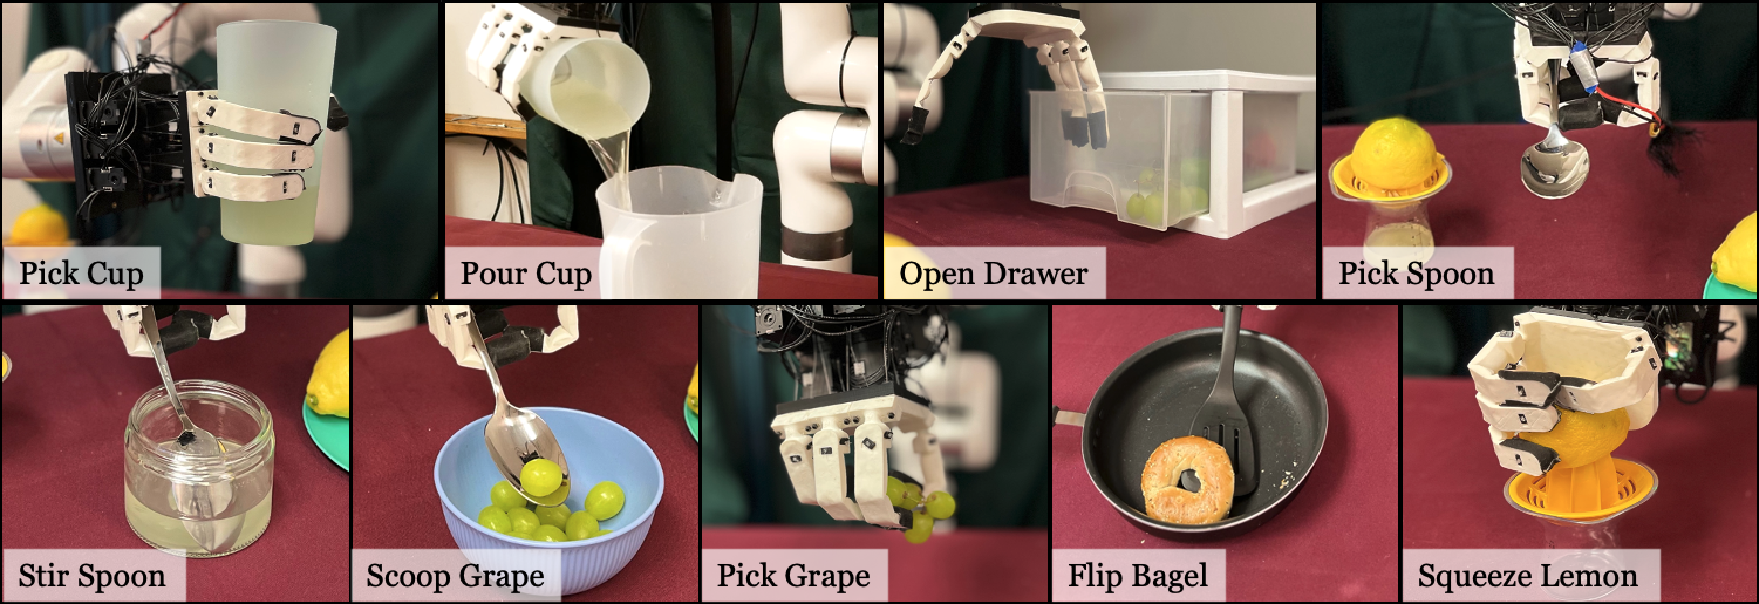
\includegraphics[width=\linewidth]{figs/teaser.pdf}
\vspace{-0.2in}
  \caption{\small We present \ours, a novel approach that can learn complex, dexterous tasks in the real world in an efficient manner. \ours manipulates tools and soft objects without any robot demonstrations.}
 \label{fig:teaser}
\end{figure}


The longstanding goal of robot learning is to build robust agents that can perform long-horizon tasks autonomously. This could for example mean a self-improving robot that can build furniture or an agent that can cook for us. A key aspect of most tasks that humans would like to perform is that they require complex motions that are often only achievable by hands--consider the task of tying shoelaces. Such a task would be impossible with a parallel jaw gripper. Therefore, in this work, we investigate real-world dexterous manipulation, its challenges, and its deployment in the real world. 

A key challenge in deploying  policies in the real world, especially with robotic hands, is that there exist many failure modes. Controlling a dexterous hand is much harder than end-effectors due to larger action spaces and complex dynamics. This problem becomes even more difficult when contacts with objects are more involved, as there can be many points of contact on a robotic hand. To address this, one option is to \textit{improve} directly in the real world via \textit{practice}. Traditionally, reinforcement learning (RL) and imitation learning (IL) techniques have been used to deploy hands-on tasks such as in-hand rotation or grasping. To be proficient at any skill a lot of practice or data is needed. This is often the case as setups are built so that it is either easy to simulate in the real world or robust to practice. However, the real world contains tasks that one cannot simulate (such as manipulation of soft objects like food) or difficult settings in which the robot cannot practice (sparse long-horizon tasks like assembly). How can we build an approach that can scale to such tasks? 

There are several issues with current approaches for practice and improvement in the real world. Robot hardware often breaks, especially with the amount of contact to learn dexterous tasks like operating tools. We thus investigate using a \textit{soft anthropomorphic hand} ~\cite{mannam2023framework}, which can easily run in the real world without failures or breaking. This soft anthropomorphic hand is well-suited to our approach as it is flexible and can gently handle object interactions. The hand does not get damaged by the environment and is robust to continuous data collection. Due to its human-like proportions and morphology, retargeting human hand grasps to robot hand grasps is made simpler.  

Unfortunately, this hand is difficult to simulate due to its softness. Directly learning from scratch is also difficult as we would like to build \textit{generalizable policies}, and not practice for every new setting.  To achieve efficient real-world learning, we must learn a prior for reasonable behavior to explore using useful actions.  Many previous methods rely on in-domain human demonstrations that are manually collected by a human operator or demonstrator \cite{shaw2022video, zhao2023learning, pomerleau1988alvinn, mandlekar2021matters}. Due to recent advances in large-scale computer vision, we propose \textit{leveraging human data to learn priors} for dexterous tasks, and improving on such priors in the real world. We aim to use the vast corpus of internet data to define this prior. What is the best way to combine human priors with online practice, especially for hand-based tasks? When manipulating an object, the first thing one thinks about is where on the object to make contact, and how to make this contact. Then, we think about how to move our hands \textit{after the contact}. In fact, this type of prior has been studied in computer vision and robotics literature as \textit{visual affordances} \cite{fouhey2015defense, bahl2023affordances, hap, hotspots, 100doh, hoi, hoi4d, wang2017binge}. In our approach, \ours, we build dexterous grasp affordances which predict the contact point, hand pose at contact, and post-contact trajectory. To improve upon these, we introduce a sampling-based approach similar to the Cross-Entropy Method (CEM) to fine-tune. Specifically, we tune the robot hand grasp, the pose, and the post-grasp trajectory all in the real world for a variety of tasks.  This method enables iterative real-world improvement in less than an hour. 

In summary, our approach (\ours) executes real-world learning on a soft robot hand with only a few trials in the real world.  To facilitate this efficiently, we train priors on human motion from internet videos. We introduce 9 challenging tasks (as seen in Figure \ref{fig:teaser}) that are difficult even for trained operators to perform: Picking a Cup, Pouring Lemonade, Opening a Drawer, Picking a Spoon, Scooping a Grape, Stirring a Spoon, Picking Grapes, Flipping a Bagel, and Squeezing a Lemon.  While our method begins to show good success on these tasks with real-world fine-tuning, more investigation is required to complete these tasks more effectively. Please see our website for details and videos at \url{http://dexterousfinetuning.github.io}.

\section{Related Work}
\label{sec:related_work}

\subsection{Real-world robot learning}
Real-world manipulation tasks can involve a blend of classical and learning-based methods. Classical approaches like control methods or path planning often use hand-crafted features or objectives and can often lack flexibility in unstructured settings \cite{karaman2011anytime, kuffner2000rrt, mukadam2016gaussian}. On the other hand, data-driven approaches such as deep reinforcement learning (RL) can facilitate complex behaviors in various settings, although these methods frequently rely on lots of data, privileged reward information and struggle with sample efficiency \cite{kober2008primitives, peters2010reps, lillicrap2015continuous,popov2017dataefficient, pathakICMl17curiosity}. Efforts have been made to scale end-to-end RL  \cite{levine2016learning, nair2018visual, agrawal2016learning, haarnoja2017sql, kalashnikov2018qt, kalashnikov2021mt} to the real world, but their approaches are not yet efficient enough for more complex tasks and action spaces and are reduced to mostly simple tasks even after a lot of real-world learning.  Many approaches try to improve this efficiency such as by using different action spaces \cite{vices2019martin}, goal relabeling \cite{her}, trajectory guidance \cite{levine2013guided}, visual imagined goals \cite{nair2018visual}, or curiosity-driven exploration \cite{mendonca2023alan}.

\subsection{Learning from Human Motion}
The field of computer vision has seen much recent success in human body and object interaction with deep neural networks.  The human hand is often parametrized with MANO, a 45-dimensional vector \cite{MANO:SIGGRAPHASIA:2017} of axes aligned with the wrist, and a 10-dimensional shape vector. MANOtorch from \cite{yang2021cpf} aligns it with the anatomical joints.   Many recent works detect MANO in monocular video \citep{wang2020rgb2hands, hmr, FrankMocap_2021_ICCV}.  Some also detect objects as well as the hand together \cite{100doh, ye2022s}.  We use FrankMocap to detect the hand for this work. 

There are many recent datasets including the CMU Mocap Database and Human3.6M \citep{ionescu2013human3} for human pose estimation, 100 Days of Hands \citep{100doh} for hand-object interactions,  FreiHand \citep{Freihand2019} for hand poses, Something-Something \citep{SomethingSomething_ICCV} for semantic interactions. ActivityNet datasets \citep{caba2015activitynet}, or YouCook~\citep{youcook} are action-driven datasets that focus on dexterous manipulation.  We use these three datasets: \citep{ego4d} is a large-scale dataset with human-object interactions, \citep{Liu_2022_CVPR} for curated human-object interactions, and \citep{EPICKITCHENS} which has many household kitchen tasks.  In addition to learning exact human motion, many others focus on learning priors from human motion. \cite{ma2022vip, nair2022r3m} learn general priors using contrastive learning on human datasets. 

\subsection{Learning for Dexterous Manipulation}
With recent data-driven machine learning methods, roboticists are now beginning to learn dexterous policies from human data as well.  Using the motion of a human can be directly used to control robots \citep{dexpilot, sivakumar2022robotic, qin2022from}. Moving further, human motion in internet datasets can be retargeted and used directly to pre-train robotic policies \citep{shaw2022video, mandikal2022dexvip}. Additionally, using human motion as a prior for RL can help with learning skills that are human-like \cite{rajeswaran2017learning, peng2018deepmimic, mandikal2021dexvip}. Without using human data as priors, object reorientation using RL has been recently successful in a variety of settings  \citep{andrychowicz2020learning, chen2022visual}.  Similar to established work in robot dogs which do not have an easy human analog to learn from, these methods rely on a lot of training data collected in simulation along with zero-shot transfer \citep{agarwal2023legged, margolis2022rapid}.

\subsection{Soft Object Manipulation}
Manipulating soft and delicate objects in a robot's environment has been a long-standing problem. Using the torque output on motors, either through measuring current or through torque sensors, is useful feedback to find out how much force a robot is applying \cite{yoshikawa1985dynamic, asada1991robot}.  Coupled with dynamics controllers, these robots can learn to not apply too much torque to the environment around them \cite{lynch2017modern, liu2017designing, khatib1987unified}.   A variety of touch sensors \cite{si2023robotsweater, yuan2017gelsight, bhirangi2021reskin, SSundaram:2019:STAG} have also been developed to  feel the environment around it and can be used as control feedback.  

Soft robotics, like our robot hand, inherently have compliant properties that make them sensitive to the environment \cite{rus2015design, wang2018toward}.  However, this introduces other difficult design challenges.  Soft materials can change properties and are difficult to manufacture.  Soft robots, including our robot hand, often do not know the end-effector tip position in a closed-loop manner \cite{butterfass2001dlr, bauer2022towards}.
\section{Background}
\label{sec:background}

\subsection{DASH: Dexterous Anthropomorphic Soft Hand}

Recently introduced, DASH (Dexterous Anthropomorphic Soft Hand)~\citep{mannam2023framework} is a four-fingered anthropomorphic soft robotic hand well-suited for machine learning research use.  We use the DASH hand on the end-effector of our arm for this work. 

The DASH hand's human-like size and form factor allows us to retarget human hand grasps to robot hand grasps easily and perform human-like grasps.  Each finger is actuated by 3 motors connected to string-like tendons, which deform the joints closest to the fingertip (DIP joint), the middle joint (PIP joint), and the joint at the base of the finger (MCP joint).  There is one motor for the finger to move side-to-side at the MCP joint, one for the finger to move forward at the MCP joint, and one for PIP and DIP joints.  The PIP and DIP joints are coupled to one motor and move dependently.  While the motors do not know the end-effector positions of the fingers, we learn a mapping function from pairs of motor angles and visually observed open-loop finger joint angles. These models are used to command the finger joint positions learned from human grasps.  

\subsection{Retargeting MANO to Soft Hand}

In order to use human hand poses as a prior for the end effector joints, we need to first detect hand poses with a model such as MANO \cite{MANO:SIGGRAPHASIA:2017}, and then develop an effective method to retarget it to soft hand joints.

For MANO parameters, the axis of each of the joints is rotation aligned with the wrist joint and translated across the hand.  However, our robot hand operates on forward and side-to-side joint angles.  To translate the MANO parameters to the robot fingers, we extract the anatomical consistent axes of MANO using MANOTorch. Once these axes are extracted, each axis rotation represents twisting (not possible for human hands), bending, and spreading.  We then match these axes to the robot hand.  The spreading of the human hand's fingers (side-to-side motion at the MCP joint) maps to the side-to-side motion at the robot hand's base joint.  The forward folding at the base of the human hand (forward motion at the MCP joint) maps to the forward motion at the base of the robot hand's finger.  Finally, the bending of the other two finger joints on the human hand, PIP and DIP, map to the robot hand's PIP and DIP joints.  While the thumb does not have anatomically the same structure, we map the axes in the same way. 

Other approaches \cite{sivakumar2022robotic} rely on creating an energy function to map the human hand to the robot hand.  However, because the soft hand is similar in anatomy and size to a human hand, it does not require energy functions for accurate retargeting.

%%% Local Variables:
%%% coding: utf-8
%%% mode: latex
%%% TeX-engine: xetex
%%% TeX-master: "../thesis"
%%% End:

\section{Fine-Tuning Affordance for Dexterity}
\label{sec:method}

\begin{figure}[H]
\centering
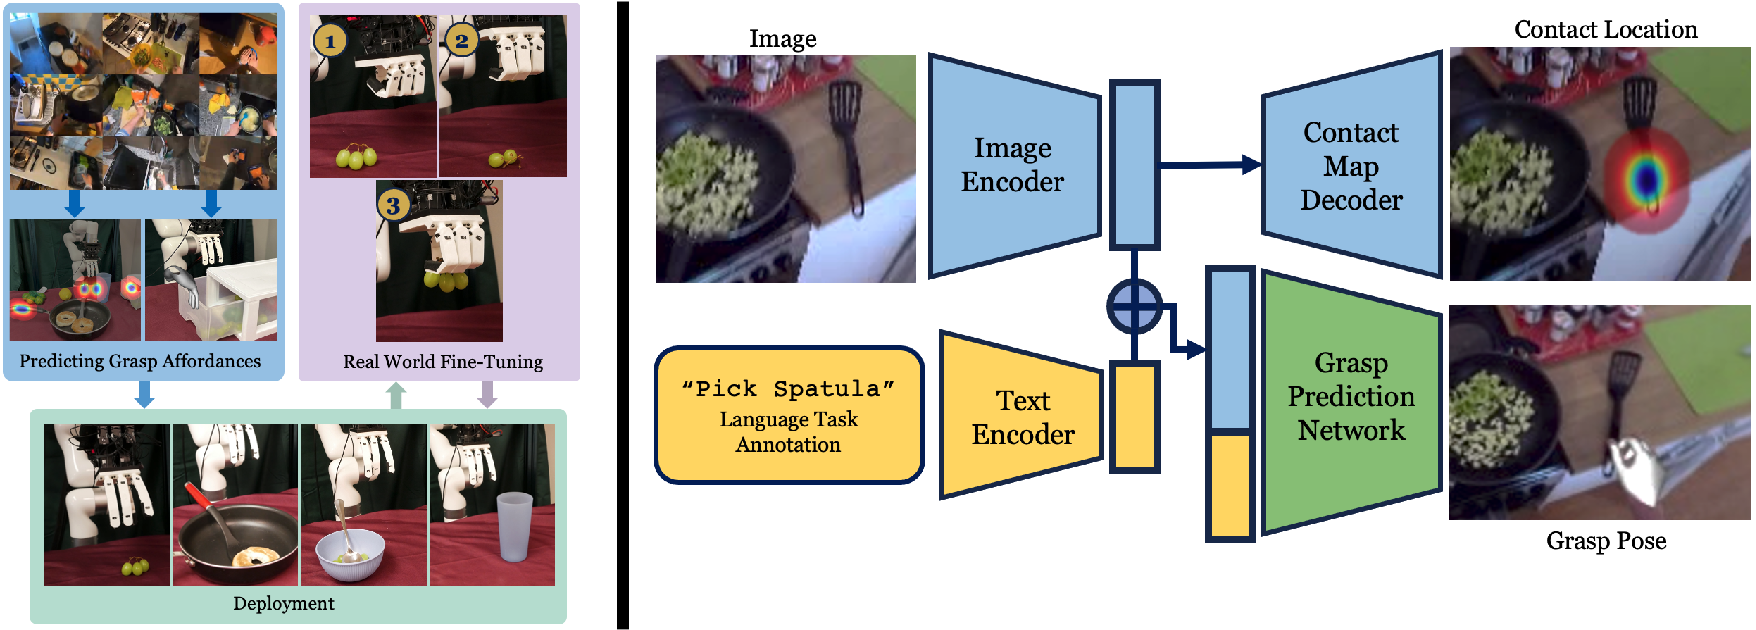
\includegraphics[width=\linewidth]{figs/method_overview.pdf}
\vspace{-0.2in}
  \caption{\small \textbf{Left:}  \ours consists of two phases: an affordance model that predicts grasp parameters followed by online fine-tuning with CEM. \textbf{Right:} Our affordance prediction setup predicts grasp location and pose.}
 \label{fig:aff_method}
 \vspace{-0.15in}
\end{figure}

The goal of \ours is to learn useful, dexterous manipulation in the real world that can generalize to many objects and scenarios.  \ours learns in the real world and fine-tunes robot hand-to-object interaction using only a few samples. However, without any priors on what is useful behavior, the robot will explore the action space inefficiently. Especially with a high-dimensional robotic hand, we need a strong prior to effectively explore the real world. We train an affordance model on human videos to learn what are reasonable behaviors the robot should perform.  

\subsection{Learning grasping affordances}
\begin{figure}[t]
\centering
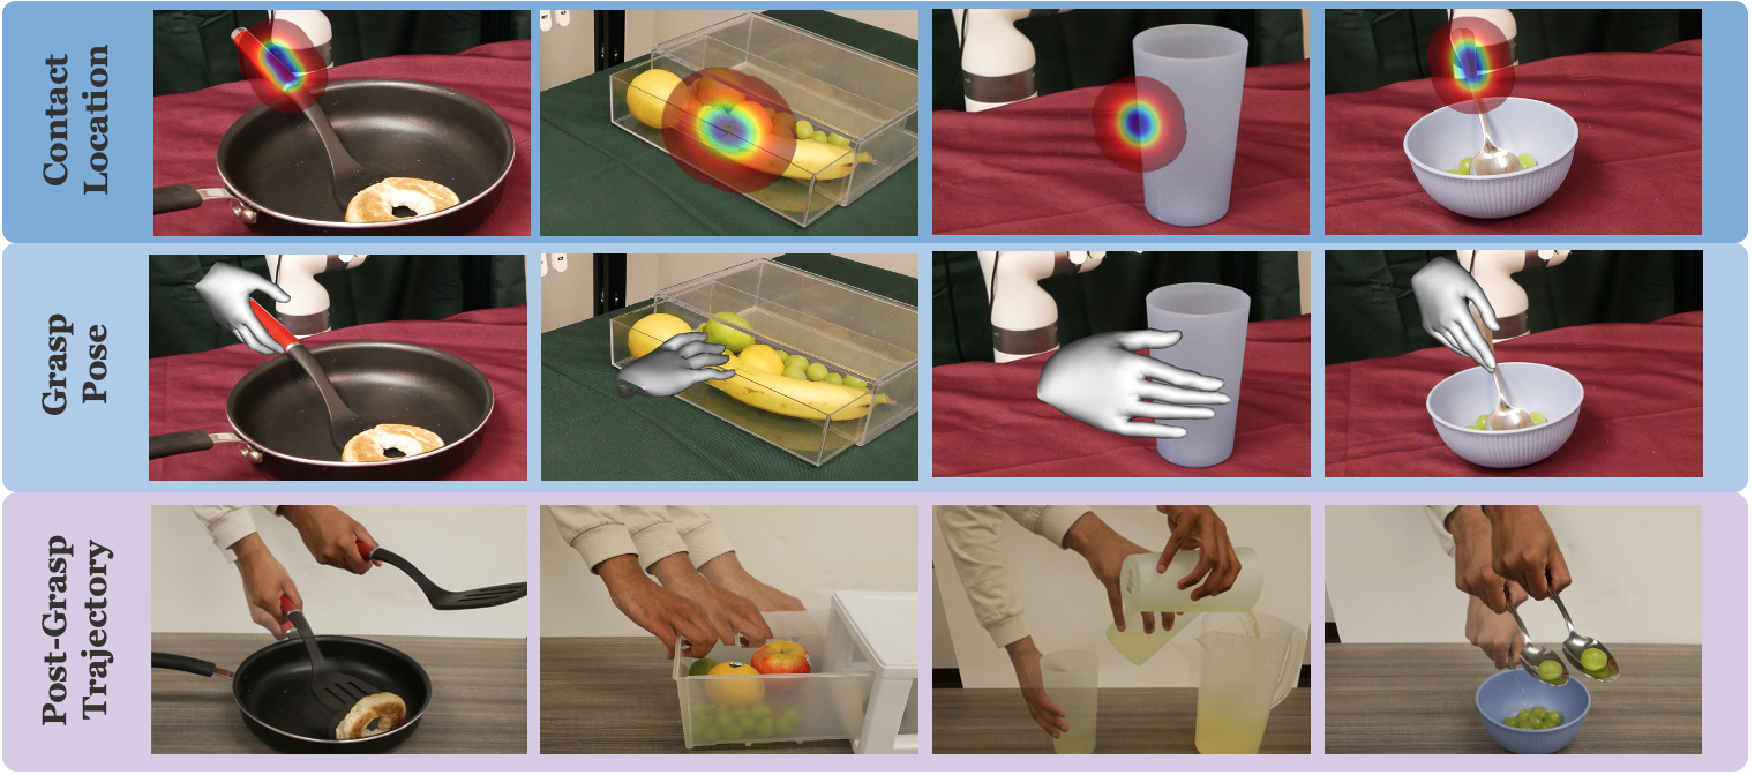
\includegraphics[width=\linewidth]{figs/aff_results.pdf}
\vspace{-0.2in}
  \caption{\small We produce three priors from human videos: the contact location (\textbf{top row}) and grasp pose (\textbf{middle row}) from the affordance prior; the post-grasp trajectory (\textbf{bottom row}) from a human demonstration of the task.}
 \label{fig:aff_results}
 \vspace{-0.15in}
\end{figure}


% \begin{wrapfigure}{l}{0.5\textwidth}
% \vspace{-0.3in}
% \begin{minipage}{\linewidth}
% \begin{algorithm}[H]
% \caption{\small Training affordances for \ours}\label{alg:cap}
% \begin{algorithmic}
% \small
% \REQUIRE Human videos $V_{1:K}$, task descriptions $T_{1:K}$, affordance model $f$. Human detection $f_\text{human}$ \citep{FrankMocap_2021_ICCV}. 

% \end{algorithmic}
% \label{algo:affordance}

% \end{algorithm}
% \end{minipage}
% \end{wrapfigure}


To learn from dexterous interaction in a sample efficient way, we use human hand motion as a prior for robot hand motion. We aim to answer the following: (1) What useful, actionable information can we extract from the human videos? (2) How can human motion be translated to the robot embodiment to guide the robot? In internet videos, humans frequently interact with a wide variety of objects. This data is especially useful in learning object affordances. Furthermore, one of the major obstacles in manipulating objects with few samples is accurately grasping the object. A model that can perform a strong grasp must learn \textit{where} and \textit{how} to grasp. Additionally, the task objective is important in determining object affordances--humans often grasp objects in different ways depending on their goal. Therefore, we extract three pieces of information from human videos: the grasp location, the human grasp pose, and the task.

Given a video clip $V = \{ v_1, v_2, \dots, v_T \} $, the first frame $v_t$ where the hand touches the object is found using a pre-trained, off-the-shelf hand-object detection model \cite{100doh}. Similar to previous approaches \cite{bahl2023affordances, hap, hoi, hotspots}, a set of contact points are extracted to fit a Gaussian Mixture Model (GMM) with centers $\mu = \{ \mu_1, \mu_2, \dots, \mu_k \}$.  Detic \cite{detic} is used to obtain a cropped image $v_1'$ containing just the object in the initial frame $v_1$ to condition the model. We use Frankmocap \cite{FrankMocap_2021_ICCV} to extract the hand grasp pose $P$ in the contact frame $v_t$ as MANO parameters. We also obtain the wrist orientation $\theta_\text{wrist}$ in the camera frame. This guides our prior to output wrist rotations and hand joint angles that produce a stable grasp. Finally, we acquire a text description $T$ describing the action occurring in $V$.

We extract affordances from three large-scale, egocentric datasets: Ego4D \cite{ego4d} for its large scale and the variety of different scenarios depicted, HOI4D \cite{hoi4d} for high-quality human-object interactions, and EPIC Kitchens \cite{EPICKITCHENS} for its focus on kitchen tasks similar to our robot's. We learn a task-conditioned affordance model $f$ that produces $(\hat{\mu}, \hat{\theta}_\text{wrist}, \hat{P}) = f(v_1', T)$. We predict $\hat{\mu}$ in similar fashion to \cite{bahl2023affordances}. First, we use a pre-trained visual model \cite{r3m} to encode $v_1'$ into a latent vector $z_v$. Then we pass $z_v$ through a set of deconvolutional layers to get a heatmap over $v_1'$ and use a spatial softmax to estimate $\hat{\mu}$.

To determine $\hat{\theta}_\text{wrist}$ and $\hat{P}$, we use $z_v$ and an embedding of the text description $z_T = g(T)$, where $g$ is the CLIP text encoder \cite{Clip}. Because transformers have seen success in encoding various multiple modes of input, we use a transformer encoder $\mathcal{T}$ to predict $\hat{\theta}_\text{wrist}, \hat{P} = \mathcal{T}(z_v, z_T)$. Overall, we train our model to optimize
\begin{align}
    \mathcal{L} = \lambda_\mu || \mu - \hat{\mu} ||_2 + \lambda_\theta || \theta_\text{wrist} - \hat{\theta}_\text{wrist} ||_2 + \lambda_P || P - \hat{P} ||_2
\end{align}


At test time, we generate a crop of the object using Segment-Anything \cite{kirillov2023segment} and give our model a task description. The model generates contact points on the object, and we take the average as our contact point. Using a depth camera, we can determine the 3D contact point to navigate to. While the model outputs MANO parameters \cite{MANO:SIGGRAPHASIA:2017} that are designed to describe human hand joints, we retarget these values to produce similar grasping poses on our robot hand in a similar manner to previous approaches \cite{handa2020dexpilot, sivakumar2022robotic}. In addition to the affordance model $f$, we collect one demo of the human doing the robot task (Figure~\ref{fig:aff_results}). This demo is used as a prior on the post-grasp trajectory.  We extract the task-specific wrist trajectory after the grasp using \cite{FrankMocap_2021_ICCV}. In the fine-tuning stage, we initialize the post-grasp trajectory with this human demonstration. Once we have this prior, how can the robot \textit{improve} upon it? 


\subsection{Fine-tuning via Interaction}

\begin{wrapfigure}{l}{0.55\textwidth}
\vspace{-0.3in}
\begin{minipage}{\linewidth}
\begin{algorithm}[H]
\caption{Fine-Tuning Procedure for \ours}\label{alg:cap}
\begin{algorithmic}
\small
\REQUIRE Task-conditioned affordance model $f$, task description $T$, post-grasp trajectory $\tau$, residual policy $\pi$. $E$ number of elites, $M$ number of warm-up episodes, $N$ total iterations. 

\FOR{$k = 1 \dots N$}
    \STATE $I_{k, 0} \gets $ initial image
    \STATE $\xi_k \gets f(I_{k, 0}, T)$
    \STATE $\epsilon_k = \pi(I_{k, 0}, \xi_k)$
    \STATE Execute grasp from $\xi_k + \epsilon_k$, then trajectory $\tau$
    \STATE Collect reward $R_k$; reset environment

    \IF{$k > M$}
        \STATE Order traj indices $i_1, i_2, \dots, i_k$ based on rewards
        \STATE $E \gets \{ \epsilon_{i_1}, \epsilon_{i_2}, \dots, \epsilon_{i_E} \} $
        \STATE Fit $\pi(.)$ as a VAE to $E$
    \ENDIF
\ENDFOR

\end{algorithmic}
\label{algo:finetune}

\end{algorithm}
\end{minipage}
\end{wrapfigure}


The affordance prior allows the robot to narrow down its learning behavior to a small subset of all possible behaviors. However, these affordances are not perfect and the robot will oftentimes still not complete the task.  This is partially due to morphology differences between the human and robot hands, inaccurate detections of the human hands, or differences in the task setup. In order to improve upon this, we practice in an online fashion to optimize the learned skills. 

Let the grasp location, wrist rotation, and grasp pose, as well as the trajectory from our affordance prior be $\xi$. During training we sample noise $\epsilon \sim \mathcal{D}$ where $\mathcal{D}$ is initialized to $\mathcal{N}(0, \sigma^2)$ (for a small $\sigma$). We rollout a trajectory parameterized by $\xi + \epsilon$. We collect $R_i$, the reward for each $\xi_i = f(v_i) + \epsilon_i$ where $v_i$ is the image.  After an initial number of $M$ warmup episodes, we rank the rollouts based on $R_i$ and extract sampled noise from the elite trajectories $\{ \epsilon_{i_1}, \epsilon_{i_2}, \dots, \epsilon_{i_k} \}$. We fit $\mathcal{D}$ to the elite trajectories to improve the sampled noise. 

At test time, we could take the mean values of the top $N$ trajectories for the rollout policy.  However, this does not account for the appearance of different objects, previously unseen object configurations, or other properties in the environment. To account for this, we train a VAE \cite{SohnNIPS2015, rezende2014stochastic, rezende2014vae, kingma2013vae} to output residuals $\delta_j$ conditioned on an encoding of the initial image $\phi(I_{j, 0})$ and affordance model outputs $\xi_j$ from the top ten trajectories. We train an encoder $q(z | \delta_j, c_j)$ where $c_j = (\phi(I_{j, 0}), \xi_j)$, as well as a decoder $p(\delta_j | z, c_j)$. At test time, our residual policy $\pi (I_0, \xi)$ samples $z \sim \mathcal{N}(\mathbf{0}, \mathbf{I})$ and predicts $\hat{\delta} = p(z, (I_0, \xi))$. Then we rollout the trajectory determined by the parameters $\xi + \hat{\delta}$.

\section{Experimental Setup}
\label{sec:setup}

\begin{figure}[H]
\centering
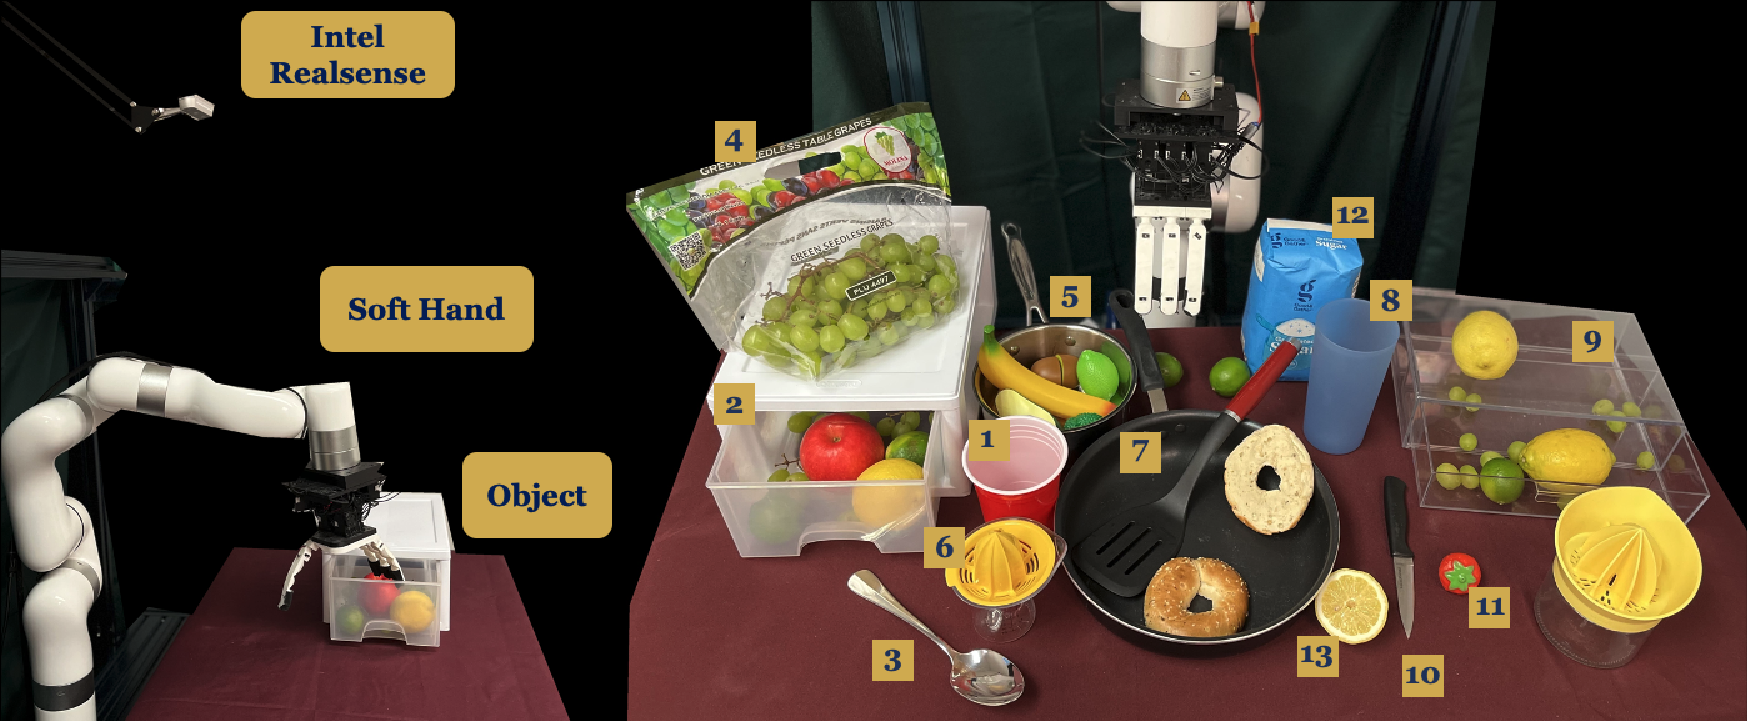
\includegraphics[width=\linewidth]{figs/workspace.pdf}
\vspace{-0.2in}
  \caption{\small \textbf{Left}: Workspace Setup. We place an Intel RealSense camera above the robot to maintain an egocentric viewpoint, consistent with the affordance model's training data. \textbf{Right}: Thirteen objects used in our experiments.}
 \label{fig:workspace}
 \vspace{-0.15in}
\end{figure}

\subsection{Task Setup} We introduce 9 tabletop tasks: \textit{Pick Cup}, \textit{Pour Cup}, \textit{Open Drawer}, \textit{Pick Spoon}, \textit{Scoop Grape}, \textit{Stir Spoon}, \textit{Pick Grape}, \textit{Flip Bagel}, and \textit{Squeeze Lemon}. For all tasks, we randomize the position of the object on the table, as well as use train and test objects with different shapes and appearances to test for generalization. See Figure~\ref{fig:workspace} for a depiction of the robot's workspace and the objects we use in our experiments.

We define the success criteria in each of our 9 tasks as follows:

\begin{itemize}
    \item Pick Cup: Cup must leave table surface and stay grasped throughout trial.
    \item Pour Cup: Cup must be grasped throughout trial and also rotate so that the top of the cup is at a lower height than the base.
    \item Open Drawer: Drawer is initially slightly open so that it can be grasped. By the end of the rollout, the drawer should be at least 1 centimeter more open than it was at the beginning.
    \item Pick Spoon: The spoon must not be in contact with the table at the end of the trial.
    \item Stir Spoon: The spoon base must rotate around the jar/pot at least 180 degrees while grasped.
    \item Scoop Grape: The spoon must have a grape at the end of the trial while being held by the soft hand.
    \item Pick Grape: All grapes must be held by the hand above the table surface. In particular, if any single grape falls due to a weak stem, this is considered a failure.
    \item Flip Bagel: The side of the bagel that is facing up at the end of the trial should be opposite the side facing up at the beginning.
    \item Squeeze Lemon: The lemon should be grasped securely on top of the juicer.
\end{itemize}

\subsection{Online Fine-Tuning Setup}

To achieve real-world learning with the soft robot hand, we pretrain an internet affordance model as a prior for robot behavior.  As explained in Section \ref{sec:method}, we train one language-conditioned model on all data.  At test time, we use this as initialization for our real-world fine-tuning. The fine-tuning is done purely in the real world.  An operator runs 10 warmup episodes of CEM, followed by 20 episodes that continually update the noise distribution, improving the policy. We train a residual VAE policy that trains on the top ten CEM rollouts to predict the noise given the image and affordance outputs. Over all our experiments, we collect data for several thousands of rollouts for over \textbf{100 hours} of real world data collection.

\subsection{Datasets and Affordance Model Parameters}

We use data from Ego4D \cite{ego4d}, EpicKitchens-100 \cite{EPICKITCHENS}, and HOI4D \cite{hoi4d}.  After filtering for clips of sufficient length, clips that involve grasping objects with the right hand, and clips that have language annotations, we used 64666 clips from Ego4D, 9144 clips from EpicKitchens, and 2707 clips from HOI4D. In total, we use a dataset of 76517 samples for training our model.

For our contact location model, we use the visual encoder from \cite{r3m} to encode the image as a 512-dimensional vector. We use the spatial features of the encoder to upsample the latent before applying a spatial softmax to return the contact heatmap. This consists of three deconvolutional layers with 512, 256, and 64 channels in that order.

To predict wrist rotation and grasp pose, we use the language encoder from \cite{Clip} to compress the language instruction to a 512-dimensional vector. We concatenate the visual and language latents and pass it through a transformer with eight heads and six self-attention layers. We pass the result of the transformer through an MLP with hidden size 576, and predict a vector of size 48: the first 3 dimensions are the axis-angle rotations; the last 45 dimensions are the joint angles of the hand. These correspond to the parameters output by Frankmocap \cite{FrankMocap_2021_ICCV}, which we used to get ground truth hand pose in all the datasets.

We jointly optimize the L2 loss of the contact location $\mu$, the wrist rotation $\theta_\text{wrist}$ and grasp pose $P$. The weights we used for the losses are $\lambda_\mu = 1.0, \lambda_\theta = 0.1, \lambda_P = 0.1$. We train for 70 epochs with an initial learning rate of 0.0002, and a batch size of 224. We used the Adam optimizer \cite{kingma2014adam} with cosine learning rate scheduler. We trained on a single NVIDIA RTX A6000 with 48GB RAM.

\subsection{Hardware Setup}

We use a 6-DOF UFactory xArm6 robot arm for all our experiments. We attach it to a 16-DOF Soft Hand using a custom, 3D-printed base. We use a single, egocentric RGBD camera in order to capture the 3D location of the object in the camera frame. We calibrate the camera so that the predictions of the affordance model can be converted to and executed in the robot frame. The flexibility of the robot hand also makes it robust to collisions with objects or unexpected contact with the environment. 

\subsection{Safety} 

In our fine-tuning experiments, there is a particular focus on the safety of the robot system and the environment. The soft hand allows the policy to perform high-contact manipulation tasks without breaking because of its compliance. Our method takes advantage of the compliance as it performs thousands of iterations in the real world.

While the end-effector is soft, the arm is not. Because it is susceptible to damage when colliding with the environment, we constrain the arm's velocity and ensure that the arm stays above the tabletop. The rollout will be terminated if the arm's dynamics controller senses that the arm collided aggressively with the environment.
 
\section{Results}
\label{sec:results}

We performs a variety of experiments to answer the following questions:  1) How good is our affordance model? 2) How well can \ours learn and improve in the real world? 3) How can the experience collected by \ours be distilled into a policy? 4) How can \ours be used for complex, soft object manipulation? We investigate the role of the affordance model and real-world fine-tuning in Table~\ref{tab:main} and Figure~\ref{fig:graph_main}. Then we perform a series of ablations in Table~\ref{tab:abl}.

\begin{table}[H]
    \centering
    \resizebox{\linewidth}{!}
    {%
        \begin{tabular}{lcccccccccccccccc}
        \toprule
        Method & \multicolumn{2}{c}{Pick cup} & \multicolumn{2}{c}{Pour cup} & \multicolumn{2}{c}{Open drawer} & \multicolumn{2}{c}{Pick spoon} & \multicolumn{2}{c}{Scoop Grape} & \multicolumn{2}{c}{Stir Spoon} & \\ 
        & train & test & train & test & train & test & train & test & train & test & train & test \\
        \midrule
        \
        \textbf{\texttt{Real-World Only}} & 0.0 & 0.1 & 0.2 & 0.1 & 0.1 & 0.0 & 0.7 & 0.3 & 0.0 & 0.0 & 0.3 & 0.0 \\ 
        \textbf{\texttt{Affordance Model Only}} & \multicolumn{2}{c}{0.1} & \multicolumn{2}{c}{0.4} & \multicolumn{2}{c}{\textbf{0.5}} & \multicolumn{2}{c}{0.5} & \multicolumn{2}{c}{0.0} & \multicolumn{2}{c}{0.3}\\ 
        
        \midrule
        \textbf{\texttt{\ours}} & \textbf{0.8} & \textbf{0.8} & \textbf{0.8} & \textbf{0.9} & \textbf{0.5} & \textbf{0.4} & \textbf{0.8} & \textbf{0.6} & \textbf{0.7} & \textbf{0.3} & \textbf{0.8} & \textbf{0.5}\\
        %%\textbf{\texttt{\ours First Iteration}} & 0.0 & 0.0 & 0.1 & 0.0 & 0.4 & 0.2 & 0.6 & 0.5 & 0.1 & 0.2 & 0.5 & 0.4\\ 
        \bottomrule
        \end{tabular}
    }
    \vspace{0.05in}
    \caption{We present the results of our method as well as compare them to other baselines: Real-world learning without internet priors used as guidance and the affordance model outputs without real-world learning.  Together, our method is able to better complete these tasks.}
    \label{tab:main}
\end{table}



\subsection{Effect of affordance prior} 
The human affordance model predicted three items: the contact location, the wrist grasp rotation, and and the hand joint pose. In the Real-World Only model, we use a few heuristics in place of each item in the affordance prior and proceed with fine-tuning. For contact location, we detect the object in the scene using a popular object detection model \cite{kirillov2023segment} and let the contact location prior be the center of the bounding box. For the wrist rotation, use a generic rotation with the pal of the hand facing downward. Finally, for the hand joint angles, we fix a half-closed hand as the grasp pose prior.  

With these heuristics, the robot has difficulty finding stable grasps consistently across a range of tasks. While the robot is able to navigate to the object, the main obstacle was finding the correct rotation angle for the hand. Hand rotation is very important for many tool manipulation tasks because it requires not only picking the tool but also grasping in a stable manner. While the soft hand shows decent success in grasping a spoon (where the grasp rotation from the heuristic is close to the correct grasp rotation) it is not able to perform well in tasks that require other wrist rotations.

It is possible that with more exploration the Real-World Only model would be able to catch up with \ours. However, we believe that these results indicate that the human affordance model reduces the number of fine-tuning iterations necessary in the real world.


\begin{figure}[t]
\centering
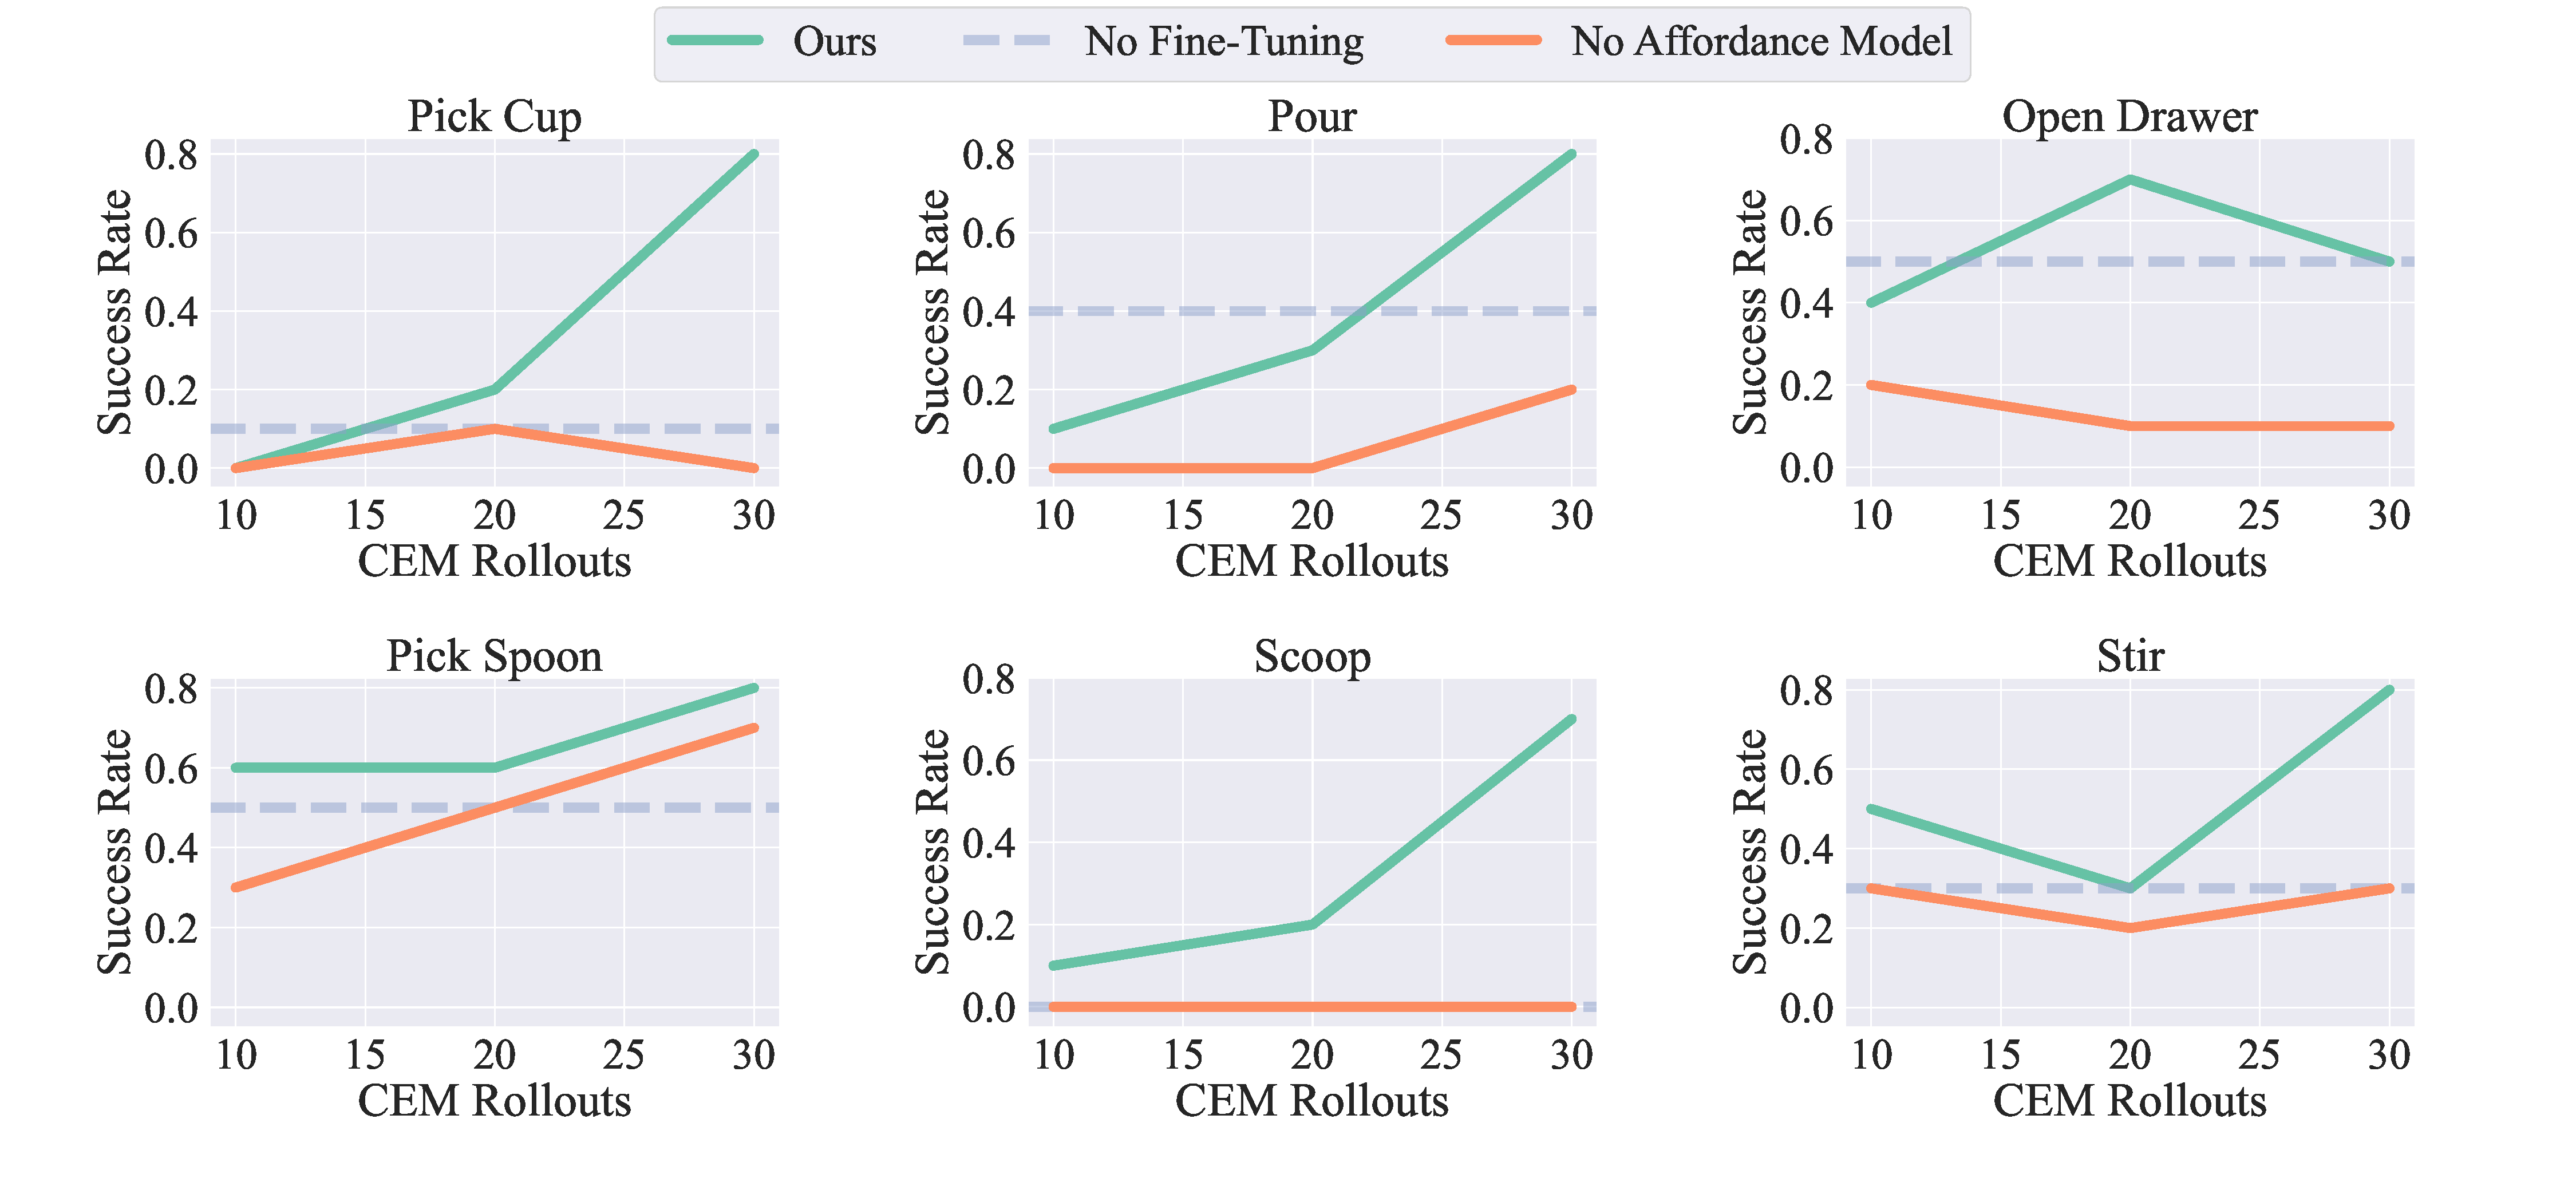
\includegraphics[width=\linewidth]{figs/graphs_main.pdf}
\vspace{-0.25in}
  \caption{\small Improvement results for 6 tasks: pick cup, pour, open drawer, pick spoon, scoop, and stir. We see a steady improvement in our method as more CEM episodes are collected.
}
 \label{fig:graph_main}
 \vspace{0.1in}
\end{figure}


\subsection{Zero-shot model execution} 
We explore the zero-shot performance of our prior with the Affordance Only model.  Without applying any online fine-tuning to our affordance model, we rollout the trajectory parameterized by the prior.  While our model performs decent on simpler tasks, the model struggles on tasks like stir and scoop that require strong, power grasps (shown in Table~\ref{tab:main}). In these tasks, the spoon collides with other objects, so fine-tuning the prior to hold the back of the spoon is important in maintaining a reliable grip throughout the post-grasp motion. Because \ours incorporates real-world experience with the prior, it is able to sample contact locations and grasp rotations that can better execute the task. 

One observation we found is that our zero-shot model sometimes performs better than the residual model trained on the first ten CEM iterations. This is due to \ours optimizing the grasp parameters only after ten iterations. Our first residual model learns only from random noise, explaining why our zero-shot performance can be stronger than \ours after few iterations of fine-tuning.


\begin{figure}[t]
\centering
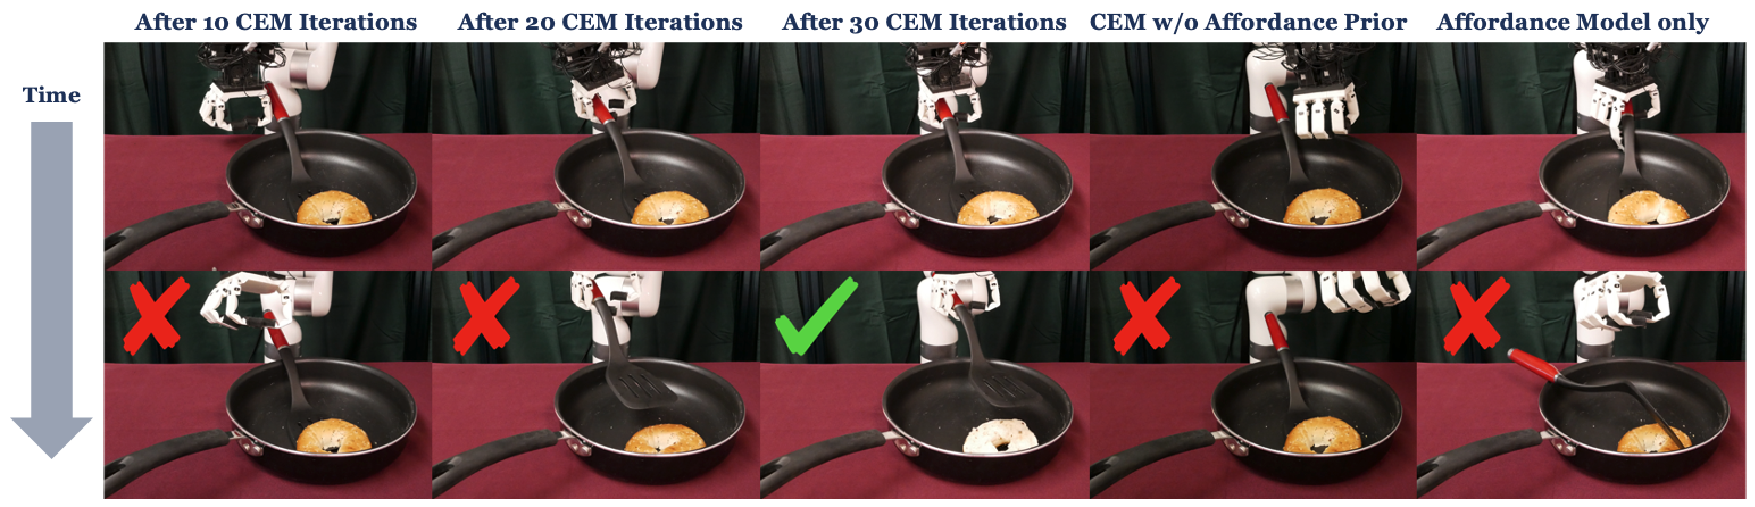
\includegraphics[width=\linewidth]{figs/qual_results.pdf}
\vspace{-0.2in}
  \caption{\small Qualitative results showing the finetuning procedure for \ours.  The model learns to hold the spatula and flip the bagel after 30 CEM iterations. }
 \label{fig:task_bagel}
 \vspace{-0.15in}
\end{figure}


\subsection{Human and automated rewards}
Our method queries the operator during the task reset process to assign a continuous score from $0$ to $1$ for the grasp.  Because the reset process requires a human-in-the-loop regardless, this adds little marginal cost for the operator.  But what if we would like these rewards to be calculated autonomously?  

We use the final image collected in the single post-grasp human demonstration from Section \ref{sec:method} as the goal image.  We define the reward to be the negative embedding distance between the final image of the rollout and the goal image with either an R3M \cite{r3m} or a ResNet \cite{resnet} encoder. The model learned from ranking trajectories with R3M reward is competitive with \ours in two of the three tasks we tested on, and performed better than the model that used Resnet18 rewards. Using a third-person camera could potentially improve the rankings because changes in the environment will be more apparent. These results indicate that using a visual reward model can potentially provide reasonable results compared to human rewards.

\begin{table}[t]
    \centering
    \resizebox{0.85\linewidth}{!}
    {%
        \begin{tabular}{lcccccc}
        \toprule
        Method & \multicolumn{2}{c}{Pour Cup} & \multicolumn{2}{c}{Open Drawer} & \multicolumn{2}{c}{Pick Spoon}  \\ 
         &train & test & train & test & train & test\\
        \midrule
        \multicolumn{2}{l}{\textit{Reward Function:}}\vspace{0.0em}\\
        \textbf{\texttt{R3M Reward}} & 0.0 & 0.0 & 0.4 & \textbf{0.5} & 0.5 & 0.4\\ 
        \textbf{\texttt{Resnet18 Imagenet Reward}} & 0.1 & 0.2 & 0.3 & 0.1 & 0.4 & 0.2\\ 
        \midrule
        \multicolumn{2}{l}{\textit{Policy Ablation:}}\vspace{0.0em}\\
        \textbf{\texttt{\ours w/ MLP}} & 0.0 & 0.0 & 0.5 & 0.0 & 0.6 & 0.5\\ 
        \textbf{\texttt{\ours w/ Transformer}} & 0.4 & 0.5 & \textbf{0.6} & 0.1 & 0.4 & 0.5\\  
        \textbf{\texttt{\ours w/ Direct Parameter est.}} & 0.1 & 0.1 & 0.1 & 0.0 & 0.3 & 0.0\\ 
        \midrule
        \textbf{\texttt{\ours }} & \textbf{0.8} & \textbf{0.9} & 0.5 & 0.4 & \textbf{0.8} & \textbf{0.6} \\ 
        \bottomrule
        \end{tabular}
    }
    \vspace{0.05in}
    \caption{Ablations for (1) reward function type, (2) model architecture, and (3) parameter estimation approach.}
    \label{tab:abl}
\end{table}


\subsection{Model Architecture} We investigate different models and training architectures for the policy trained on the rollouts (Table~\ref{tab:abl}). When we replace the conditional VAE with an MLP that predicts residuals, the model has difficulty learning the grasp rotation to effectively pour a cup. This may be because VAEs can compress multi-modal data more effectively (which is useful for our case as our data includes location, rotation, and joint angles).

Our transformer ablation is an offline method similar to \cite{chen2021decisiontransformer} where in addition to the image and affordance model outputs, we condition on the reward outputs and train a transformer to predict the residual. At test time the maximum reward is queried and the output is used in the rollout. We hypothesize that the reduced performance is because the transformer is a data-hungry architecture. The model may need more real-world data, which can be expensive to collect.

Finally, we train a VAE to directly estimate $\xi$ instead of the residual. This model was unable to effectively distill the information from the affordance prior with neither the diversity of data nor training time allotted. As a result, it often makes predictions that are far from the correct grasp pose. 


\begin{figure}[t]
\vspace{-0.2in}
\begin{center}
    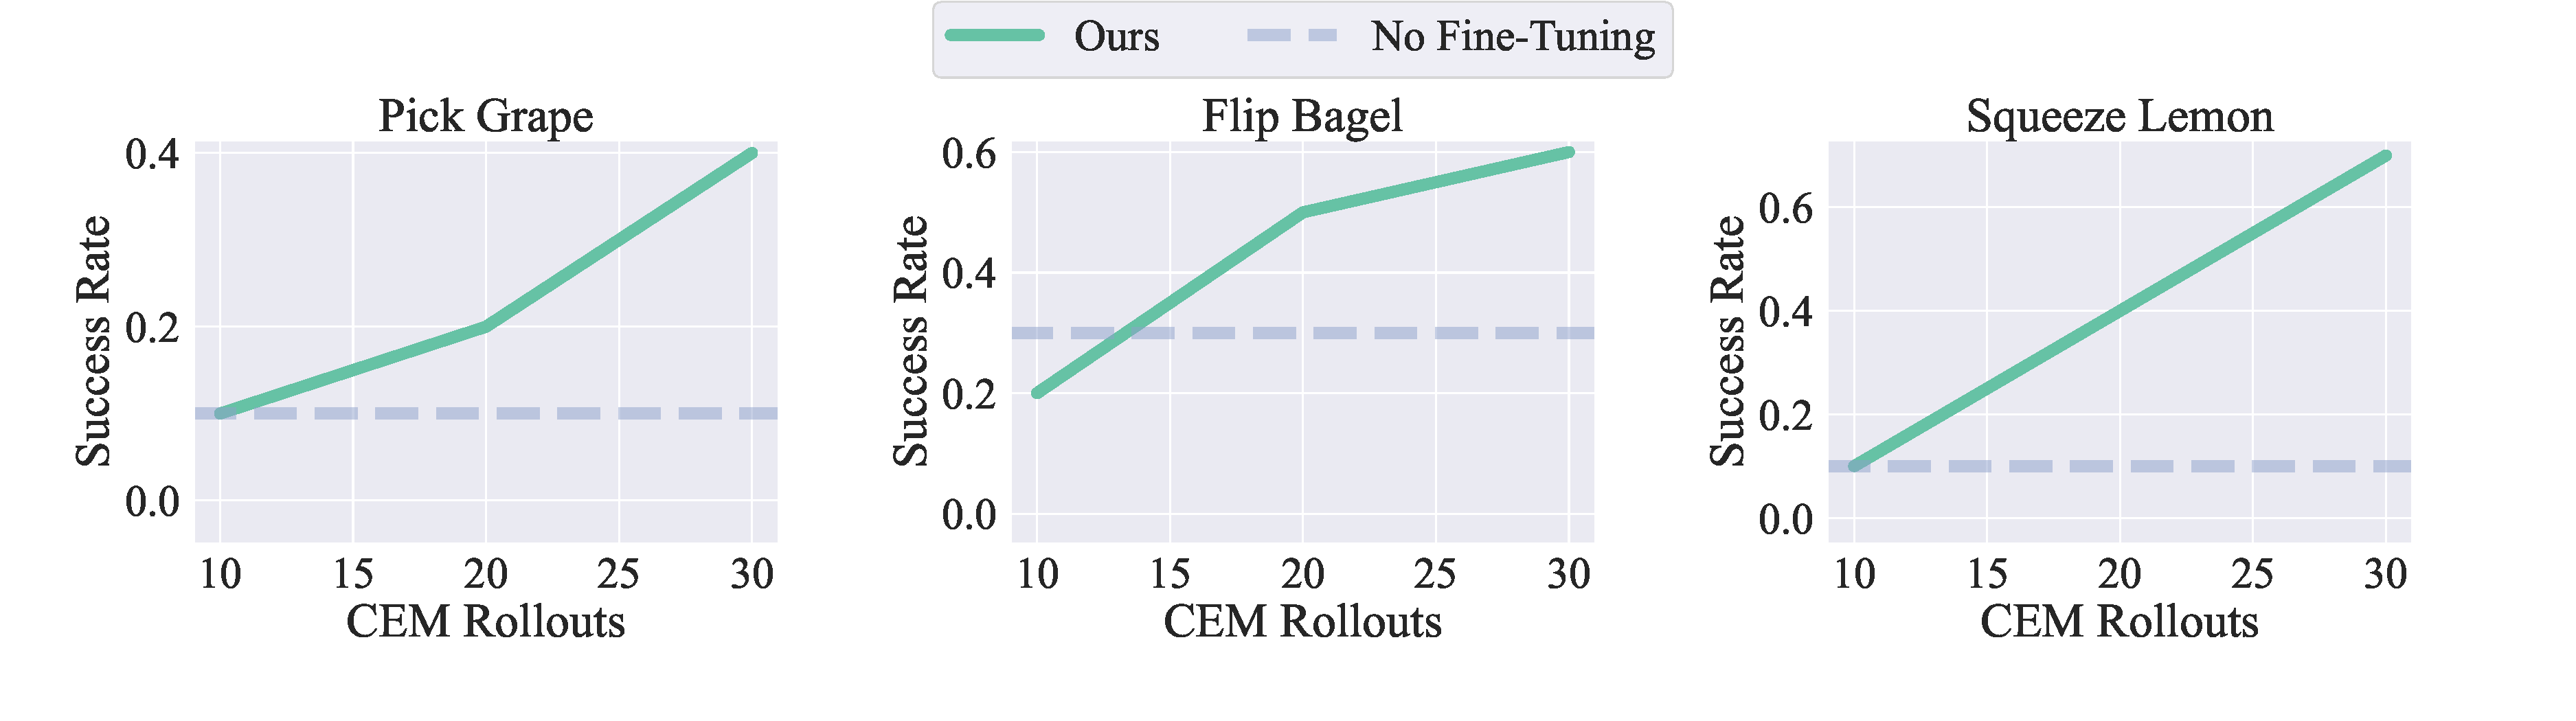
\includegraphics[width=\linewidth]{figs/graphs_difficult.pdf}
\end{center}
\vspace{-0.1in}
  \caption{\small We evaluate \ours on three additional difficult manipulation tasks. }
 \label{fig:graph_difficult}
 \vspace{-0.15in}
\end{figure}


\subsection{Performance on complex tasks and soft objects} 
We investigate the performance of \ours on more challenging tasks, which involve grasping or manipulating food. Tasks involving soft objects cannot be simulated accurately, so sim2real methods may have difficulty performing these tasks in the real world. Our method does not have that challenge in this setting and \ours is able to perform reasonably well on these tasks.

Of the three tasks, our method has the most difficulty with the Pick Grape task. This is because grapes are small and require the fingers to curl fully to maintain a stable grasp. A limitation of our hand is that the range of MCP joint does not allow the fingertips to touch its palm, and as a result it has difficulty in consistently picking small objects.

\section{Discussion and Limitations}
\label{sec:discussion}

In this thesis, we investigate how to learn dexterous manipulation in complex setups. \ours aims to learn directly in the real world. In order to efficiently perform real world fine-tuning, we build an \textit{affordance} prior learned from human videos. We are able to practice and improve in the real world via our online fine-tuning approach, enabled by the use of a soft anthropomorphic hand, performing a variety of tasks (involving both rigid and soft objects).

However, there are some limitations to our work.  While we are able to learn policies for the high-dimensional robot hand, the grasps learned are not multi-modal and do not capture all of the different grasps humans are able to perform.  In particular, we find that the predicted hand poses are all power grasps, which is used even in situations where other grasps might be more appropriate (such as a pinch grasp when picking a grape). We believe that this is mainly caused by noisy hand detections. As these detection models improve, we hope to be able to learn a more diverse set of hand grasps. 

Second, during finetuning, resets require human input and intervention. This limits the amount of real-world learning we can do, as the human has to be constantly in the loop to reset the objects. Other works \cite{chen2022single, guptaYuZhaoKumar2021reset} introduce paradigms that might potentially be useful in helping scale our method for more fine-tuning iterations.

Third, the arm has additional physical limitations. While the DASH hand is soft like the human hand, the robot arm is rigid. As a result, the robot cannot mimic \textit{every} grasp humans make. For example, any underhand grasp that involves sliding the hand underneath an object is not possible with this setup because the arm would collide with the table. A soft arm would enable a wider range of human-like grasps.

Finally, the soft hand's fingers do not curl fully. The soft hand's fingers have a tradeoff between the strength and range of motion. The version of the soft hand used for the experiments in this project has high strength, which is useful to pick large, heavier objects. However, this makes grasping smaller objects, such as individual grapes, more difficult. A hand that can have the best of both worlds would facilitate a larger variety of tasks and is a potential area for future research.

\chapter{Zero-Shot Rewards from Human Videos}
\label{cha:reward}

\section{Introduction}
\label{sec:intro_reward}

Despite recent advances in robot learning, there are many challenges in advancing towards the long-standing goal of developing generalist robotic agents. To achieve this objective, one must develop a framework that can generalize across diverse environments, tasks, and robot embodiments. Perhaps the most concise way to represent these challenges is the problem of learning a goal-conditioned reward function. Critically, we want to learn and deploy a reward function in a way that is amenable to different tasks and environments.

Traditionally, designing a robotic agent to perform tasks in the real world using reinforcement learning has proved difficult due to the sheer amount of data that needs to be collected in the process of exploring the environment. As a result, much of the advancement in reinforcement learning has come from model-free reinforcement learning in simulated environments. Whereas NLP and vision research has shown greater generalization when scaling to large datasets \cite{gpt3}, the collection and use of large, task-specific data in robot learning has encountered more challenges due to the physical cost of robot deployment. Collecting robot data at scale must provide guarantees for safety, and it requires human supervision for task resets. Many robots are trained in a single environment on a small number of tasks. 

Rather than attempting to collect robot interaction data, a growing body of work has focused on exploiting the abundance of internet data, particularly ego-centric video, inspired by the success of CLIP \cite{radford21clip}. The vast quantity of human manipulation data available online could be a useful prior for robot manipulation. In particular, the diversity of the environments and tasks depicted in internet-scale data could improve generalization when learning a goal-specific reward function. With this in mind, many recent works have collected labelled, in-the-wild, egocentric videos of humans manipulating objects and performing various tasks \cite{ego4d, smthsmth, epickitchens}.

However, there are two immediate challenges in utilizing offline human videos for learning a reward function. Firstly, there is a difference in embodiments when training with human data compared to test time where trajectories are generated in the robot's action space. Transferring rewards across this embodiment gap is necessary to learn a robot policy. Secondly, there is often a difference between human and robot trajectories in environment and visual appearance of the agents in the scene. 

What is the best way to learn a reward representation in the absence of robot data? Our approach to learn a reward function is to mask and inpaint over the agent in a visual scene to provide agent-agnostic data alignment. In visually removing the agent from the scene, we hope to learn a reward representation that focuses on relevant, environment-centric features of the scene that are modified over the course of the trajectory. With the diversity of environments in datasets like Something-Something \cite{smthsmth} and Ego4D \cite{ego4d}, we believe that we can learn generalizable reward functions across different robotic tasks in simulation environments. Additionally, with this approach we wish to use only human demonstrations in specifying a goal. In particular, due to our focus on building an agent-agnostic reward function, we investigate only the zero-shot paradigm: no robot demonstrations are used in learning a policy.

We demonstrate that our method shows promise on several tasks in a simulated environment with a Sawyer arm. More investigation is required to scale this method to a diverse range of tasks.
\section{Related Work}
\label{sec:related_work_reward}

\subsection{Reward Learning}

While many works have used Reinforcement Learning (RL) with great success \cite{silver2017alphago, Vinyals2019GrandmasterLI, rma, agarwal2023legged}, RL assumes access to a reward function which may not always be easy to define or optimize for. Inverse RL is the field for defining reward functions from demonstrations and has many prior work \cite{ziebart2008maximum, ratliff2006mmp, wulfmeier2015DeepIRL, levine2018maxent}. Many ecent works have aimed to generalize to scenarios where humans provide desired outcomes \cite{fu2018variational, singh2019end}. However, these works aim to learn rewards in single-task settings. Our work concentrates on the multi-task setting, where we hope to learn a reward function that generalizes to many tasks. In particular, we wish to learn a function that can generate rewards for many tasks given one human demonstration per task.


\subsection{Pre-training Representations for Control} 

A natural approach to address multi-tasks generalization is pre-training on large datasets. Indeed, many works  leverage large-scale data to pre-train representations for control \cite{Parisi2022TheUE, Cui2022CanFM, r3m, VIP, shah2021rrl, radasavovic22robotmaskedpretraining}. To create generalized image representations, some have trained on a wide variety of images to take advantage of the natural supervision that’s abundantly available on the internet \cite{radford21clip}. Many works have adopted these universal embeddings for downstream robotics tasks \cite{shridhar2022cliport, jang2022bc}. Others have combined language embeddings with human videos to learn representations that can be used for robot manipulation tasks \cite{shao2021concept2robot}. Similarly, \cite{r3m} applies time contrastive learning \cite{sermanet18timecontrastive}, video-language alignment \cite{nair2021lorel}, and applies a sparsity penalty to learn a robust representation from Ego4D \cite{ego4d}. This representation can in turn be utilized as a distance function for rewards.

Self-supervised representation learning from unlabeled videos encodes semantic and geometric understanding of diverse actions to define reward functions for reinforcement learning. Self-supervised representation learning from images has seen significant progress in recent years \cite{pathak2016context, chen2020simclr, caron2021dino, MAE, BYOL}, approaching the performance of fully supervised methods on ImageNet \cite{russakovsky2014imagenet}. Given the success of representation learning in the image domain, recent works adapt similar approaches for learning from video for downstream robotics applications \cite{srinivas2020curl}. \cite{radasavovic22robotmaskedpretraining} trains a single masked autoencoder \cite{MAE} on diverse, in-the-wild videos. This unified vision policy is then adapted for downstream control, significantly outperforming CLIP. \cite{sermanet18timecontrastive} proposes a time-contrastive approach learning approach from multi-view video, where different views of a robot action at the same timestamp are close in feature space, while temporally offset views should be repelled in feature space. \cite{schmeckpeper20rlvideos} directly incorporates videos collected by humans by adding videos to the replay buffer and directly performing RL on the observational data. Combining offline data with in-domain data boosts performance in the environment. \cite{zakka21xirl} addresses the generalization across agents by training representations using a cycle-consistency loss by learning from other agents demonstrating the same task that are robust to differences in shape, action, end-effector, and dynamics. 


\subsection{Robot Learning from Human Videos} 

Because collecting robot demonstrations can be costly, many works have proposed using human data, which is both plentiful and easily accessible on the internet. In recent years, many large-scale annotated human datasets have been collected, such as Something-Something \cite{SomethingSomething_ICCV}, Ego4D \cite{ego4d}, EpicKitchens \cite{epickitchens}, YouCook \cite{youcook}, and ActivityNet \cite{caba2015activitynet}. Instead of learning an intermediate representation, some works directly learn from unstructured human videos \cite{bahl22whirl, shaw2022video, bahl2023affordances}.

Other works train representations \cite{r3m, radasavovic22robotmaskedpretraining, VIP, radford21clip} that use human data. For example, VIP \cite{VIP} casts representation learning from human videos as an offline goal conditioned reinforcement learning problem to create a temporally smooth embedding for novel tasks. \cite{tian21functionaldistances} learns a visual dynamics model as well as a dynamical distance function to be used for downstream tasks. However, these approaches require a goal image with the robot at test time.

There are other methods that do not require in-domain goals by learning a classifier \cite{shao2021concept2robot, DVD}. DVD \cite{DVD} trains a discriminator to determine if two videos are performing the same task by learning from in-the-wild videos of humans. The learned feature representation can be used as a reward function for downstream robot control. However, DVD still requires in-domain robot rollouts in training to learn reward functions for downstream tasks. In our work, we build upon DVD and aim to do away with robot demonstrations at both training and test time.


\section{Zero-Shot Rewards from Human Videos}
\label{sec:method_reward}

We aim to learn a multi-task reward function by learning from human demonstrations. For each task $\mathcal{T}_i$, the reward function $\mathcal{R}$ will be conditioned on one of $K$ human demonstrations $\mathcal{D}_i = \{ d_{i,j} \}_{j=1}^K$ specifying the desired task. 

Then, given the robot environment's state space $\mathcal{S}^r$, action space of the robot $\mathcal{A}^r$, and robot dynamics $f^r(s' | s, a)$, we want to solve the MDP parameterized by $(\mathcal{S}^r, \mathcal{A}^r, f^r, \mathcal{R})$ for a task $\mathcal{T}_i$.

\begin{figure}[H]
\centering
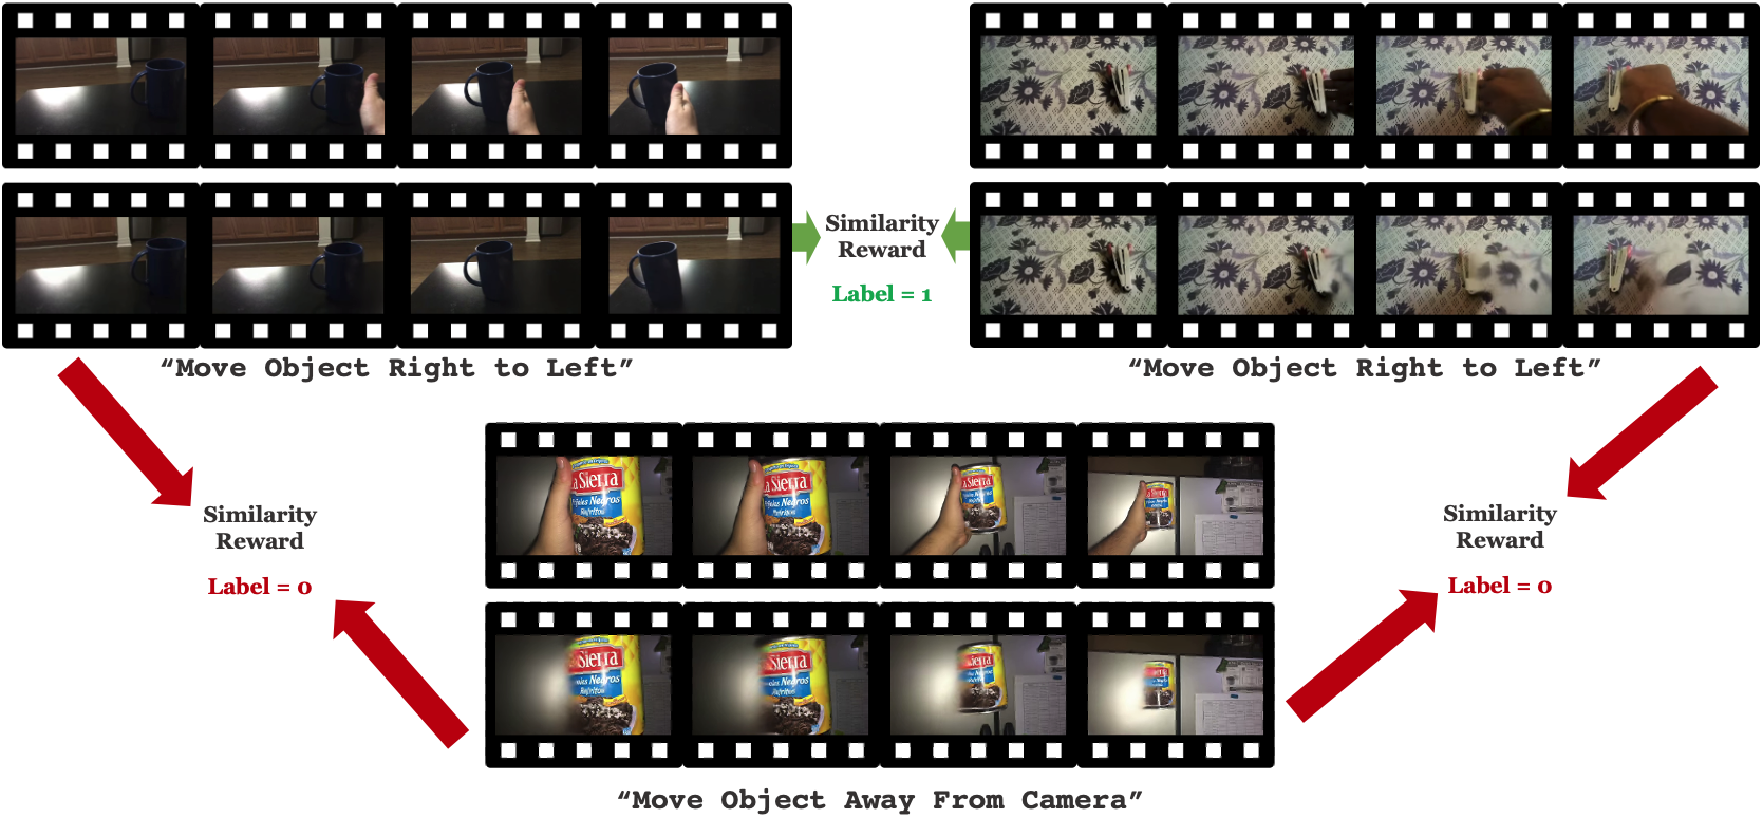
\includegraphics[width=\linewidth]{figs_reward/method_overview.pdf}
\vspace{-0.2in}
   \caption{\small Method Overview: Human data is processed as follows. We generate masks for human arms and hands in videos from the Something-Something dataset \cite{smthsmth}. Videos that do not have high quality masks are discarded. The remaining videos are inpainted based on their masks. We take this set of inpainted human videos and learn a discriminator to capture the functional features of the video. At test time, we take as input a set of human demonstrations of the same task. Using trajectories sampled from CEM, we use our reward function to judge the similarity between every (demo, trajectory) pair. We use CEM to optimize this reward function to generate trajectories that are most functionally similar to the demos.}
    \label{fig:method_reward}
    \vspace{-0.15in}
\end{figure}

\subsection{Learning Agent-Agnostic Representations}

Our work addresses the embodiment gap by visually removing the agent from the scene at both training and test time. There are a few potential inpainting methods we can use when given masks to remove the agent (human or robot) from a video. To generate the masks for the robot arm, we used Detectron2 \cite{detectron2}, a state-of-the-art segmentation method and fine-tuned it for detecting our robot. However, we found Detectron2 to be unreliable in detecting human hands and arms in egocentric data. We believe this is because Detectron2 was trained on third-person views of humans where most of the body is in the scene. For masking human hands and arms in human videos, we use EgoHOS \cite{egohos}, a method trained on egocentric videos from datasets like Ego4D \cite{ego4d} and Epic-Kitchens \cite{epickitchens}. 

While this method provides more consistent masks, there are still videos that have few or noisy masks due occlusion or difficult lighting conditions. We refine our dataset by removing videos where fewer than half of frames have human masks. This removes only one-fifth of our dataset, so we still keep a large majority of our data for training.

For inpainting, we considered two types of methods. We can utilize a video inpainting method such as Copy and Paste Networks \cite{cpnetworks} or E2FGVI \cite{e2fgvi}. Another option for inpainting is to inpaint frame-by-frame, such as with Stable Diffusion \cite{stablediffusion}. We found that video inpainting methods perform better as they have access to context for occlusions that singular images do not have. Stable Diffusion also requires many denoising iterations that reduce its speed.

\subsection{Addressing Visual Domain Gap}

While training on a large dataset with a variety of objects, lighting, and poses will provide some generalization, we conjecture that it might not be sufficient to generalize to simulation environments, which look significantly different from the real world. As a result, we account for the visual differences between simulation and real world settings. In particular, we use Stable Diffusion \cite{stablediffusion}, a pre-trained image-text generative model, to create synthetic videos by augmenting existing videos from the dataset.

To augment a video, we take individual frames from the video and generate a novel set of frames. We guide this image-to-image translation using text conditioning. That is, given a text prompt $T$ and video $V$, for each frame $ v_1, v_2, \dots, v_n \in V$ we use Stable Diffusion as a function $g$ to map it to new frame $v'_i = g(v_i, T)$. Because we are concerned specifically with generalization to simulation environments, we use prompts $T$ such as \verb|"OpenGL style rendering"|, and \verb|"Unity style rendering"| that would encourage the output frames to match the desired style.

Because this approach generates a video by transforming individual frames, this does not necessarily maintain the temporal consistency of the video. In order to keep the videos coherent, we restrict the noise added to individual frames to be sampled within a reasonable range for each video.

\subsection{Reward Training}
The reward function we want to learn is $\mathcal{R} (s_{1:T}, \mathcal{D}_i)$. Here, for each task $\mathcal{T}_i$, we have a set of human demonstrations $\mathcal{D}_i$.

We will use a pretrained inpainting method $\phi^h$ for human inpainting and $\phi^r$ for robot inpainting. During training, we can apply $\phi^h$ to each demonstration and train the DVD encoder $f_{\text{enc}}$ and similarity function $f_{\text{sim}}$ as described in their paper \cite{DVD}.

To briefly summarize the training method in DVD, we train $\mathcal{R}$ as follows. We use a pretrained encoder $f_{\text{enc}}$ and a learned similarity function $f_{\text{sim}}$ to generate the pairwise reward:

$$\mathcal{R}(d_i, d_j) = f_{\text{sim}}(f_{\text{enc}}(\phi^h(d_i)), f_{\text{enc}}(\phi^h(d_j))).$$

When learning $\mathcal{R}$ at training time, note that $f_{\text{enc}}$ and $\phi^h$ are pretrained and frozen. To learn $f_{\text{sim}}$, we sample videos $d_i^1, d_i^2, d_j \in \mathcal{D}$. We minimize the cross-entropy loss below:

$$\mathcal{L} = \mathbb{E}_{(d_i^1, d_i^2, d_j) \sim \mathcal{D}} [\log (\mathcal{R}(d_i^1, d_i^2)) + \log (1 - \mathcal{R}(d_i^1, d_j)]$$

Note that this is essentially contrastive loss over demonstrations from different tasks. Above, $d_i^1$ is the anchor, $d_i^2$ is a positive sample and $d_j$ is the negative sample.

\subsection{Task Execution}

At test time, we are given a set of human demonstrations $\mathcal{D}_i = \{ d_{i,j} \}_{j=1}^K$ for a specific task. We have a reward function $\mathcal{R}$ that can take in a robot trajectory $s_{1:T}$ and a single human demonstration $d_{i, j}$. We calculate the reward with the corresponding inpainting function, as follows:

$$\mathcal{R}(s_{1:T}, d_{i, j}) = f_{\text{sim}}(f_{\text{enc}}(\phi^r(s_{1:T})), f_{\text{enc}}(\phi^h(d_{i, j})))$$

We can optimize for this reward function using zeroth order methods like Cross-Entropy Method (CEM) or Model Predictive Path Integral (MPPI) control. For our method, we implement CEM. CEM keeps track of a trajectory distribution parameterized by a Gaussian for each action $a_i \sim \mathcal{N}(\mu_i, \sigma_i)$ for $i = 1 \dots T$. CEM then takes multiple samples from this distribution and retains the samples (elites) with the largest rewards to update the distribution for the next iteration. Then from this distribution, CEM rolls out a trajectory to act out an episode.

For the results in Table~\ref{table:baseline_comparison_reward}, we use the ground truth dynamics from the simulator when rolling out samples taken from the action distribution. We can also potentially use a state or visual dynamics function such as \cite{hafner2019dreamer} learned in the environment to run CEM efficiently in closed loop.


\subsection{Datasets and Environments}

We generate results in Metaworld \cite{metaworld}, with a tabletop environment that has a mug, drawer, and a faucet. We train our models using the Something-Something dataset \cite{smthsmth}, an egocentric dataset of humans manipulating different objects according to various tasks. We primarily evaluate our method on three tasks: \textit{Close Drawer}, \textit{Push Mug Away}, and \textit{Move Mug Right}. We train on a dataset of around 10K videos which are labelled with task information. This dataset consists of data for 6 tasks, of which three are the evaluation tasks specified above.
\section{Experiments}
\label{sec:experiments_reward}

Our experiments aim to answer the following: (1) How effectively does our method perform without any prior knowledge of robot embodiment or robot demonstrations? (2) How does our method compare to previous work? (3) Does domain augmentation improve simulation performance? (4) Does our method improve when trained on additional tasks?

\begin{figure}[H]
\centering
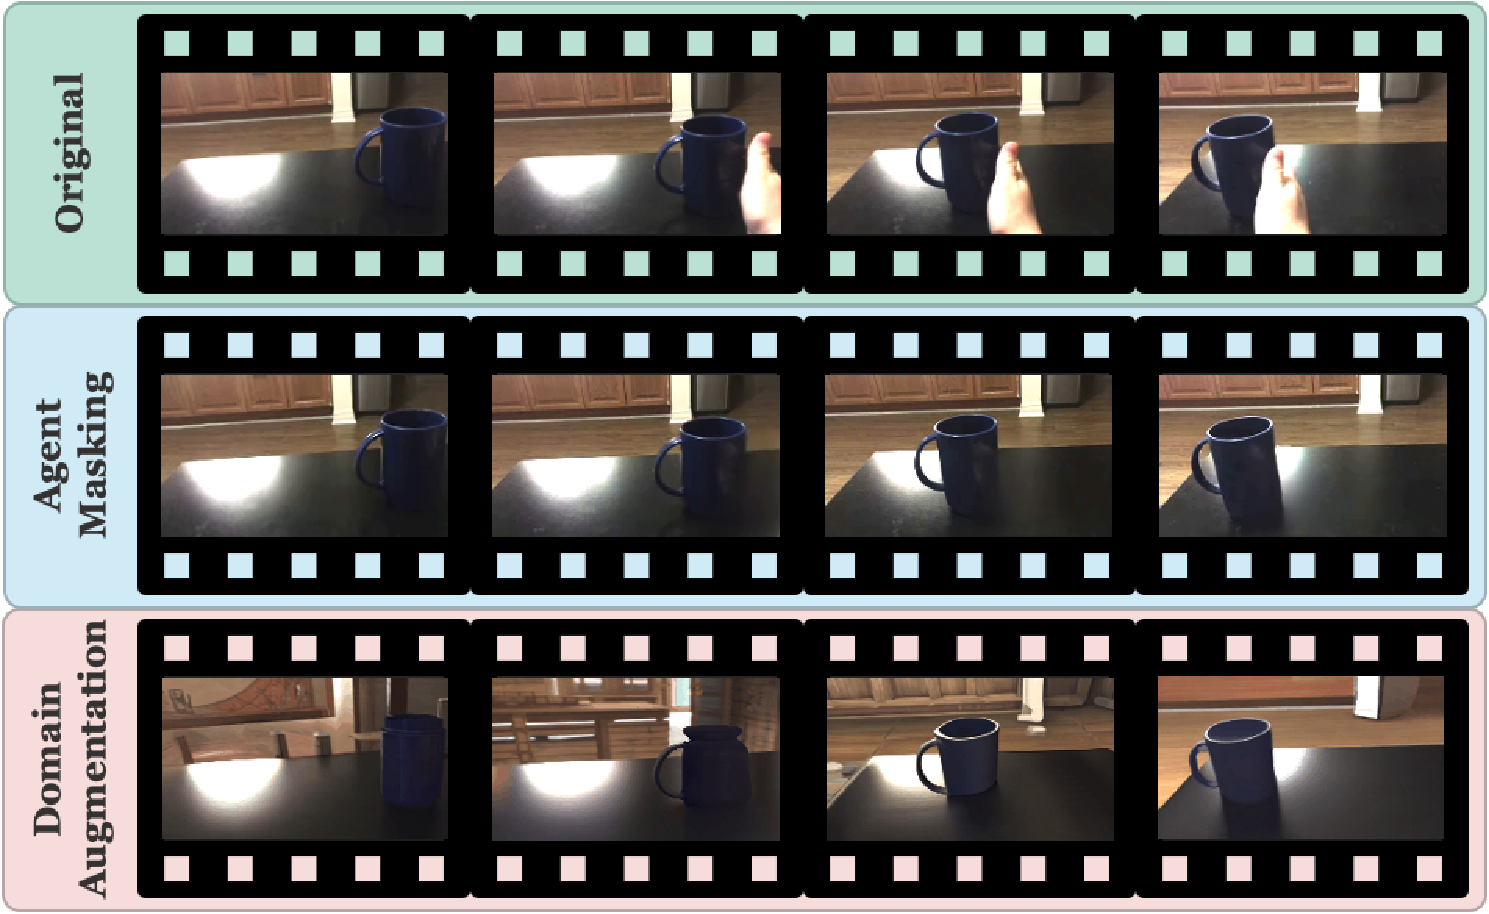
\includegraphics[width=\linewidth]{figs_reward/qual_results.pdf}
\vspace{-0.2in}
   \caption{\small Qualitative Outputs: We show the intermediate results of (1) removing the agent and (2) modifying the background with pre-trained text-to-image models.}
    \label{fig:qual_outputs_reward}
    \vspace{-0.15in}
\end{figure}

\subsection{Comparison to Prior Work}

We use two prior works as baselines: DVD \cite{DVD} and VIP \cite{VIP}. DVD's results involve training on both human and robot videos, so we hypothesize that training only on human videos is not sufficient for learning policies for robots at test time. The DVD reward function does not generalize to unseen robot embodiments. Methods like VIP that pretrain on diverse human datasets generate a reward that represents a distance function to a goal image in the robot's environment. However, we only produce human demonstrations at test time, so we hypothesize this approach will not work well either.

Our results for these baseline methods are in Table \ref{table:baseline_comparison_reward}. The methods we show results for are as follows:

\begin{itemize}
    \item \verb|Shaped Reward|: A human-specified reward function that is shaped for each task.
    \item \verb|DVD-HR|: The original implementation of DVD, trained on both human and in-domain robot demonstrations.
    \item \verb|DVD-H|: A modified version of DVD that is limited to training on only human data.
    \item \verb|VIP|: Using VIP with a goal image from an OOD human video at test time.
\end{itemize}

In the first two rows, privileged information is available for the reward function (either a manually shaped reward or robot demonstrations are available). When DVD does not have access to in-domain robot data, there is a significant decline in performance in the zero-shot setting. The DVD model struggles to learn a reward function that can transfer to the robot's environment without robot demonstrations. In practice, we see that it only performs one task, even when given demos of other tasks. VIP also does not perform well because it requires a goal image in the robot's setting.

The results of our method are also depicted in Table~\ref{table:baseline_comparison_reward}. We present our method with and without visual domain augmentation. Both reward functions perform strongly on all three tasks despite not having seen the environment in the training data or at test time. Our method performs significantly better than DVD-H and VIP in the zero-shot setting. Our method even outperforms DVD-HR on two of the three tasks. Overall, we believe that removing the agent encourages the representations learned by our method to more accurately match the functional meaning of the task by focusing on the changes in the environment. Accordingly, our method can perform better than models like DVD-HR.

\begin{table}[t]
    \centering
    \resizebox{\linewidth}{!}
    {%
        \begin{tabular}{lcccc}
        \toprule
        Model & Close Drawer & Push Mug Away & Move Mug Right & Average \\
        \midrule\midrule
        Shaped Reward & 0.99 & 0.95 & 0.99 & 0.98 \\
        DVD-HR \cite{DVD} & 0.75 & 0.59 & 0.06 & 0.47 \\
        \midrule
        \textit{Human-only Reward Functions}: \\
        DVD-H \cite{DVD} & 0.0 & 0.62 & 0.0 & 0.21 \\
        VIP \cite{VIP} & 0.09 & 0.22 & 0.14 & 0.15 \\
        \midrule
        Ours & 0.65 & 0.96 & 0.75 & 0.79 \\
        Ours + Domain Augmentation & 0.84 & 0.96 & 0.88 & 0.89 \\
        \bottomrule
        \end{tabular}
    }
    \caption{Fraction of successful iterations for each model with varying data used at training and test time. Each model was averaged over 10 different seeds, each seed being run for 100 CEM iterations.}
    \label{table:baseline_comparison_reward}

    \vspace{-0.3cm}
\end{table}

\subsection{Effect of visual domain augmentation}

As shown in Table~\ref{table:baseline_comparison_reward}, domain augmentation with Stable Diffusion improves the results of our method on two of the three tasks. Overall, it has an 89\% success rate while our method without augmentation has a success rate of 79\%. With domain augmentation, our method beats DVD-HR in all three tasks and is moving closer to the performance of the shaped reward. Our method with domain augmentation performs the zero-shot baselines by 68\%. Even though Stable Diffusion is not trained on robotics-related data, it is able to provide meaningful priors to enhance training and potentially improve generalization.

More aggressive augmentation could potentially improve the amount of generalization, but could also reduce the temporal consistency of the video as a whole. For sample augmentation outputs, see Figure~\ref{fig:qual_outputs_reward}.

\subsection{Number of Training Tasks}

\begin{figure}[t]
\vspace{-0.2in}
\begin{center}
    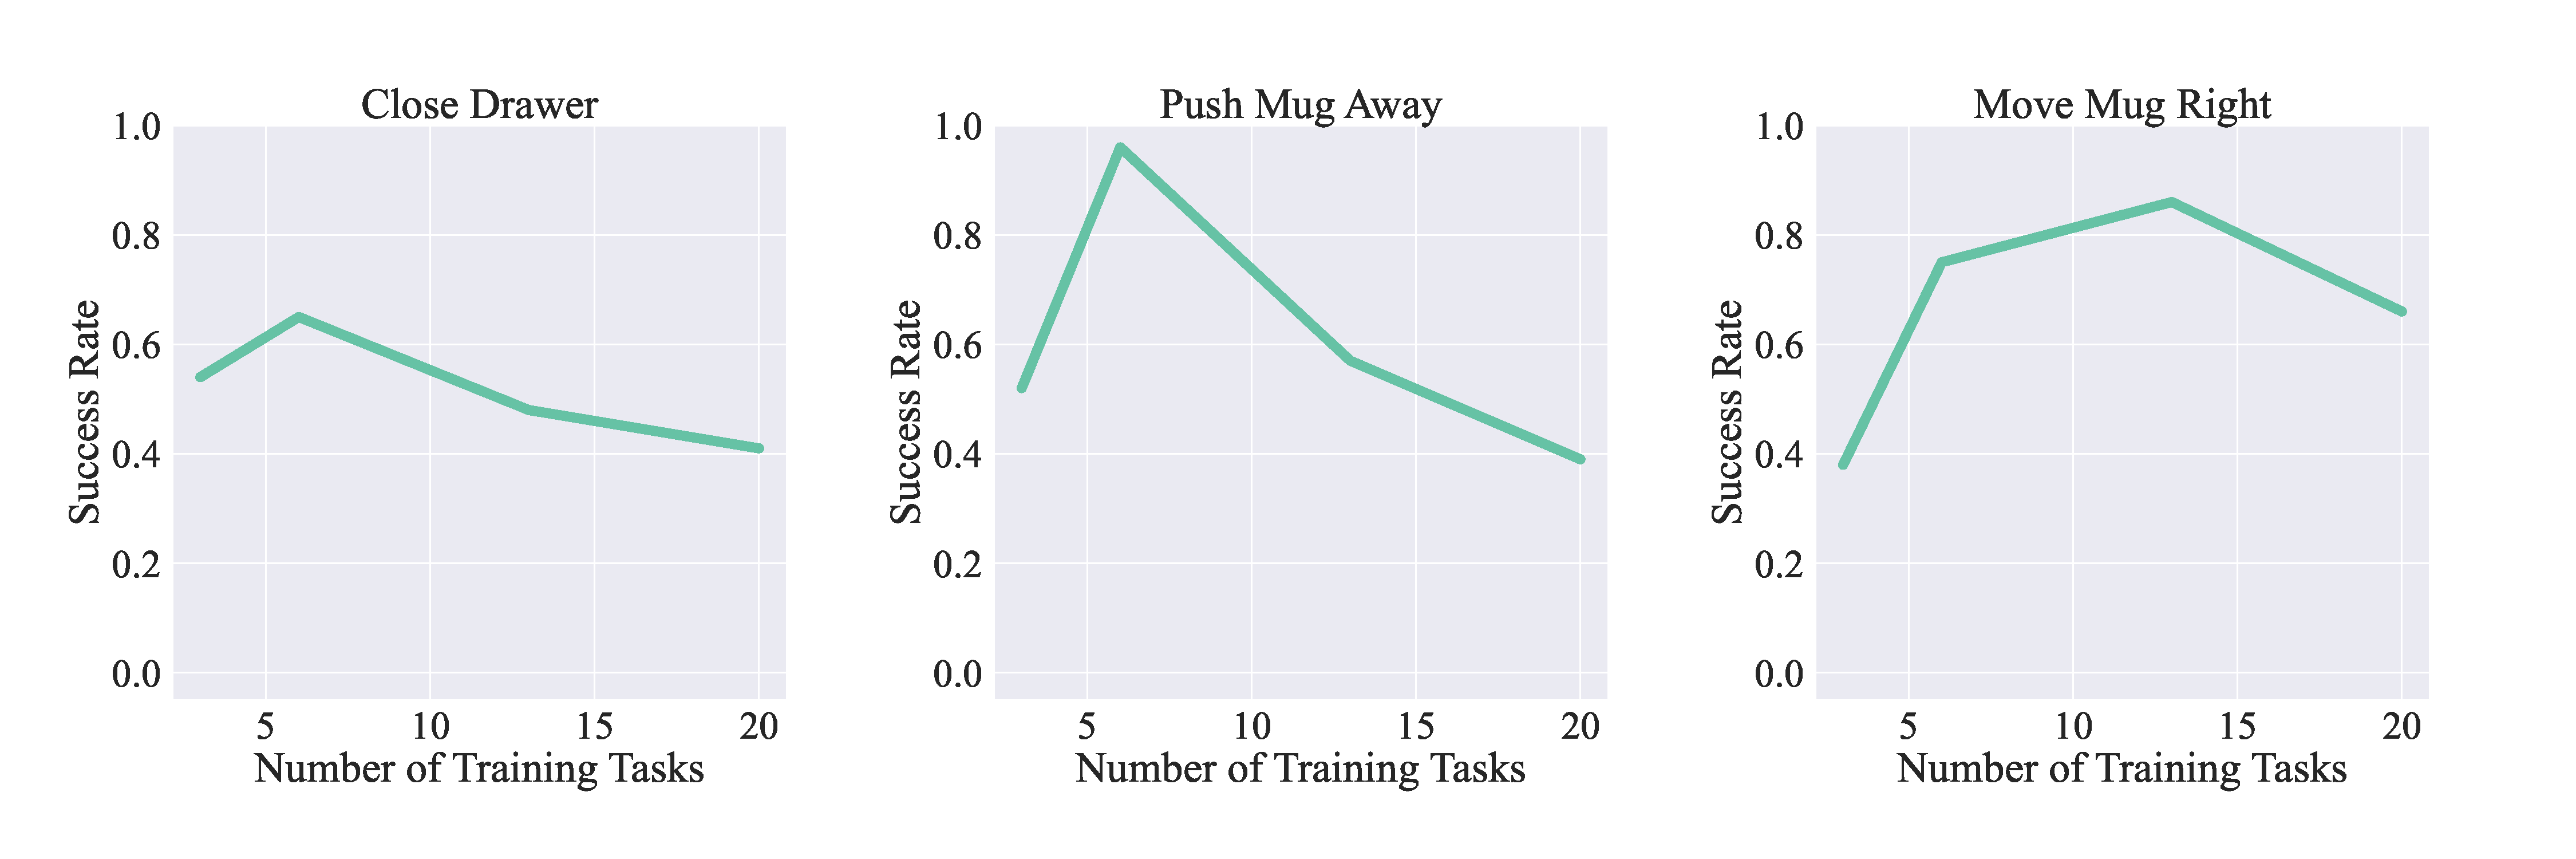
\includegraphics[width=\linewidth]{figs_reward/graph_task_ablation.pdf}
\end{center}
\vspace{-0.1in}
  \caption{\small We investigate how adding unrelated tasks in training affects the downstream performance of our method.}
 \label{fig:graph_task_ablation_reward}
\end{figure}

\begin{table}[t]
    \centering
    \resizebox{\linewidth}{!}
    {%
        \begin{tabular}{lcc}
        \toprule
        Task & Our Method (6 Task Training) & Our Method (20 Task Training) \\
        \midrule
        Close Drawer & 0.65 & 0.41 \\
        Push Mug Away & 0.96 & 0.39 \\
        Move Mug Right & 0.75 & 0.66 \\
        Move Mug Left & 0.65 & 0.31 \\
        Pull Mug to Camera & 0.01 & 0.06 \\
        Open Drawer & 0.25 & 0.0 \\
        \midrule\midrule
        Average & 0.55 & 0.31 \\
        \bottomrule
        \end{tabular}
    }
    \vspace{0.05in}
    \caption{Fraction of successful iterations for reward models trained with a varying number of tasks.}
    \label{table:more_tasks_reward}
\end{table}


The results that we described in the previous section involve training on 6 tasks. One question we wish to answer is how does the number of tasks we train on affect the performance of the reward function on robotic tasks? In other words, how does the diversity of the training data affect the quality of the reward function learned, and do unrelated videos enhance the reward function learned?

To investigate this, we additionally train a reward function with our method with 3 tasks, 13 tasks, and 20 tasks. All of these variations include the three evaluation tasks in the training set. We evaluate the 4 reward functions with the three original evaluation tasks. We show these results in Figure~\ref{fig:graph_task_ablation_reward}. We also show results comparing our method with 6 task training and 20 task training on 3 additional evaluation tasks in Table~\ref{table:more_tasks_reward}.

Based on the results in Figure~\ref{fig:graph_task_ablation_reward}, we find that scaling to more tasks in training produces better performance and generalization up to a point. The 3-task reward function performs worse than the 6-task reward function is that there are fewer total videos for training. While both models are trained for the same number of epochs, the number of videos in each epoch is smaller for the model trained with three tasks.

However, after 6 tasks, the success rate plateaus and decreases when going to 13 and then 20 training tasks. This is additionally reflected in Table~\ref{table:more_tasks_reward} where the 20-task model performs worse on all 6 evaluation tasks. This is likely due to the structure of the reward model: as the discriminator needs to be able to distinguish between more tasks, it might struggle to disambiguate the salient features for the evaluation tasks compared to the other tasks it is trained on. As a result, our method loses robustness when training on \textit{too many} unrelated tasks.

\section{Conclusion and Limitations}
\label{sec:conclusions_reward}

We presented a method building on DVD \cite{DVD} to create a reward function that is both domain-agnostic and agent-agnostic. Masking and removing the agent is an effective method to force a reward function to learn representations for tasks that involve the behavior of manipulated objects in the scene. We found that using data augmented by pretrained text-image models can further improve the robustness of the reward function at test time. Overall, our method shows promise in learning a reward function that does not rely on prior robot knowledge.

Our method also has several limitations. The core limitation of our approach is that as we train on more tasks, our model has worse performance in evaluation. Ideally, when we train on more tasks, the performance should improve slightly if not stay the same. Currently, we treat training a reward function as a binary classification problem, and this can be improved to account for similarities between similar tasks. Injecting this semantic knowledge via language embeddings would hopefully lead to a more smoother representation space that might be more effective at improving with more tasks.

Another limitation of our reward is that it is sparse. While reward functions that use the full video have additional context, it lacks the structure to evaluate partial trajectories and is sparse, unlike image-based reward functions. A reward function that evaluates partial trajectories--perhaps subvideos segmented by \textit{subgoals}--might be able to combine the best of both worlds.

Our data augmentation setup also has room for improvement. To maintain the coherency of the synthetic data generated by the model, we restricted the extent to which we augmented the frames in the video. Perhaps with more text-video generation models being open-sourced as of late, we can modify the style more aggressively while also maintaining consistency across frames. This would potentially allow for better generalization.

\chapter*{Bibliography}
\addcontentsline{toc}{chapter}{Bibliography}

\vspace{-25mm}
This bibliography contains \total{citenum} references.
\vspace{10mm}

\printbibliography[heading=none]

\end{document}

%%% Local Variables:
%%% coding: utf-8
%%% mode: latex
%%% TeX-engine: xetex
%%% End:
